\documentclass[9pt,twocolumn,twoside]{rilabRxiv}
% Use the documentclass option 'lineno' to view line numbers
\setlength{\marginparwidth}{2cm}
\usepackage[textsize=tiny,colorinlistoftodos]{todonotes} % comments in margins
\usepackage{rotating}
\definecolor{cornflowerblue}{rgb}{0.39, 0.58, 0.93}
\usepackage{multicol}


%%%%%%%Add comments in color
\newcommand{\ms}[1]{{\small \textcolor{green}{#1}}}
\newcommand{\jri}[1]{{\small \textcolor{red}{#1}}}
\newcommand{\citex}[1]{{\small \textcolor{red}{CITE(#1)}}}
\newcommand{\X}{{\textcolor{red}{X}}}

\newcolumntype{b}{X}
\newcolumntype{s}{>{\hsize=.5\hsize}X}

% Set supplement numbers to S and start counting newly
\newcommand{\beginsupplement}{%
        \setcounter{table}{0}
        \renewcommand{\thetable}{S\arabic{table}}%
        \setcounter{figure}{0}
        \renewcommand{\thefigure}{S\arabic{figure}}%
     }


\usepackage{hyperref}

\title{The temporal dynamics of background selection in non-equilibrium populations}

\author[1,$\ast$]{Raul Torres}
\author[2,$\ast$]{Markus G Stetter}
\author[3,4]{Ryan D Hernandez}
\author[5]{Jeffrey Ross-Ibarra}

\affil[1]{Biomedical Sciences Graduate Program, University of California San Francisco, San Francisco, CA, USA}
\affil[2]{Botanical institute, University of Cologne, Cologne, Germany}
\affil[3]{Department of Bioengineering and Therapeutic Sciences, University of California San Francisco, San Francisco, CA, USA}
\affil[4]{Department of Human Genetics and Genome Quebec Innovation Center, McGill University, Montreal, Canada}
\affil[5]{Department of Human Genetics of Evolution and Ecology, Genome Center, and Center for Population Biology, University of California, Davis, CA, USA}

\keywords{demography, background selection, linked selection}

\runningtitle{Demography and background selection} % For use in the footer

%% For the footnote.
%% Give the last name of the first author if only one author;
% \runningauthor{FirstAuthorLastname}
%% last names of both authors if there are two authors;
% \runningauthor{FirstAuthorLastname and SecondAuthorLastname}
%% last name of the first author followed by et al, if more than two authors.
\runningauthor{Torres, Stetter \textit{et al.}}


%%% Abstract %%%%%%%%%%%%%%%%%%
\begin{abstract}
Neutral genetic diversity across the genome is determined by the complex interplay of mutation, demographic history, and natural selection. While the direct action of natural selection is limited to functional loci across the genome, its impact can have effects on nearby neutral loci due to genetic linkage. These effects of selection at linked sites, referred to as genetic hitchhiking and background selection (BGS), are pervasive across natural populations. However, only recently has there been a focus on the joint consequences of demography and selection at linked sites, and empirical studies have sometimes come to apparently contradictory conclusions. In order to understand the relationship between demography and linked selection, we conducted an extensive forward simulation study of BGS under a range of demographic models. We found that levels of diversity compared to an equilibrium population vary  over time, and that the initial dynamics after a population size change are often in the opposite direction of the long-term expected trajectory. Our detailed observations of the temporal dynamics of neutral diversity in the context of selection at linked sites in nonequilibrium populations provides new intuition about why patterns of diversity under BGS vary through time in natural populations and helps reconcile previously contradictory observations.
Most notably, our results highlight that classical models of BGS are poorly suited for predicting diversity in nonequilibrium populations.
\end{abstract}
%%%%%%%%%%%%%%%%%%%%%%%%%%

\setboolean{displaycopyright}{false}
\hypersetup{draft} %to prevent annoying \pdfendlink error during drafting, remove for final draft (and cross fingers the error doesn't arise)
\begin{document}
\begin{multicols}{1}
\maketitle
\end{multicols}
\thispagestyle{firststyle}
%\firstpagefootnote
\correspondingauthoraffiliation{
Department of Evolution and Ecology, University of California, Davis, CA, USA
E-mail: rossibarra@ucdavis.edu \\
Department of Human Genetics, McGill University, Montreal, Canada
E-mail: ryan.hernandez@me.com\\
\textsuperscript{a} Authors contributed equally.
}
\vspace{-11pt}%


\section{Introduction}
\lettrine[lines=2]{\color{color2}T}{}
he effects of natural selection and demography on neutral genetic diversity within populations have long been of interest in evolutionary and population genetics.
Recent efforts in sequencing tens of thousands of genomes across a multitude of species have yielded new and valuable insights into how these two forces of evolution have shaped extant patterns of genomic variation.
Yet, while the theoretical underpinnings of the effects of natural selection and demography on genetic diversity have been investigated for decades \citep{smith1974hitch, nei1975bottleneck, maruyama1984population, maruyama1985population, kaplan1989hitchhiking, charlesworth1993effect, nordborg1996effect, hudson1995deleterious, tajima1989effect}, detailed investigation into how they jointly act to create patterns of diversity in different populations remains lacking.

Both theory and empirical observation have long shown that patterns of neutral genetic variation can vary regionally across the genome as a function of recombination rate \citep{smith1974hitch, begun1992levels}.
This is because natural selection operating on selected sites not only decreases genetic variation at the focal site but can also lead to decreases in nearby neutral genetic diversity due to genetic linkage \citep{cutter2013genomic}.
These effects, known as genetic hitchhiking \citep{smith1974hitch} (in which neutral variants rise to high frequency with adaptive variants) and background selection \citep{charlesworth1993effect} (BGS; in which neutral variants are removed along with deleterious variants) can be widespread across the genome \citep{elyashiv2016genomic}.
Evidence for selection at linked sites has been found across an array of species, including \textit{Drosophila melanogaster} \citep{begun1992levels, comeron2014background, charlesworth1996background, andolfatto2007hitchhiking, sella2009pervasive, elyashiv2016genomic}, mice \citep{keightley2018understanding}, wild and domesticated rice \citep{flowers2011natural, xu2012resequencing}, \textit{Capsella} \citep{williamson2014evidence}, monkeyflowers \citep{stankowski2018tempo}, maize \citep{beissinger2016recent}, and humans \citep{sabeti2002detecting, reed2005fitting, voight2006map, mcvicker2009widespread, cai2009pervasive, hernandez2011classic, lohmueller2011natural}.

Demographic change can also impact patterns of diversity across the genome.
For example, neutral theory predicts that the amount of genetic diversity is proportional to a population’s effective population size (\textit{$N_e$}), such that changes in \textit{$N_e$} should result in concomitant changes to diversity \citep{kimura1983neutral}.
However, evidence suggests that such diversity also varies much less in magnitude across species when compared to their census population sizes \citep{lewontin1974genetic, leffler2012revisiting}.
One of the most common forms of a population size change is a population bottleneck, whereby populations suffer a large decrease followed by an expansion.
Bottlenecks can occur via domestication events \citep{doebley2006molecular, tang2010domestication, wiener2011deciphering, gaut2018demography}, seasonal or cyclical fluctuations in population size \citep{elton1924periodic, ives1970further, itoh2009seasonal, noren2014genetic}, and founder events \citep{david1988genetic, dlugosch2008founding, henn2012great}.
Notably, while the rate of loss of diversity in response to a population contraction is quite fast, the recovery of diversity following a population increase can be quite slow \citep{charlesworth2009effective}.
As a result, large contemporary populations may still yield patterns of low average genetic diversity if their population size was much smaller in the recent past.
In humans, this is clearly evident in European and Asian populations due to the out-of-Africa bottleneck \citep{10002015global}.

Because selection at linked sites and demography are both pervasive forces across a multitude of species, the characterization of how these two forces interact with one another is necessary in order to develop a full picture on the determinants of neutral genetic diversity.
The efficiency of natural selection scales proportionally with \textit{$N_e$} and the impact of selection at linked sites on neutral diversity is likely to be greater in larger populations and lower in smaller populations (although the rate of change for lowered diversity may diminish as populations reach larger and larger sizes; \citet{kaplan1989hitchhiking, cutter2013genomic, corbett2015natural, gillespie2001population, santiago2016joint}).
Further, demographic changes can also increase (in the case of bottlenecks) or decrease (in the case of expansions) the rate of drift.
It is therefore plausible that the rate at which diversity at a neutral locus is perturbed by selection at linked sites could be highly dependent on both the current as well as long-term $N_e$ of the population.
This competition between the strength of selection at linked sites (which increases with N) and genetic drift (which decreases with N) may be a key contributor to the limited range of diversity observed among species  despite much larger observed differences in census size \citep{gillespie2001population, corbett2015natural, santiago2016joint}.
However, selection at linked sites alone may not be sufficient to explain the observed discrepancy between observed diversity and census populations sizes \citep{coop2016does}, and the action of both demography and selection at linked sites in concert may provide a better model. 
Moreover, the heterogeneous structure of selection at linked sites across the genome may yield different responses to demography and population splits through time and their resulting effects on patterns of differentiation and divergence also remain largely unexplored \citep{burri2017interpreting}.

Many models of selection at linked sites were also formulated with the assumption that the population is large enough (or selection strong enough) such that mutation-selection balance is maintained \citep{charlesworth1993effect, zeng2013coalescent, nicolaisen2013distortions}.
However, non-equilibrium demographic change may break such assumptions and forces other than selection may drive patterns of variation in regions experiencing selection at linked sites.
For example, during the course of a population bottleneck, genetic drift may transiently dominate the effects of selection at many sites such that traditional models of selection will poorly predict patterns of genetic diversity.
Additionally, in regions affected by selection at linked sites, the impact of genetic drift may also be exacerbated, resulting in greater losses to diversity than expected by the action of demography alone.
A recent review by \citet{comeron2017background} included a cursory investigation into the impact of demography on diversity in regions under BGS and suggested a dependency on demographic history.
Recent empirical work in maize and humans has also demonstrated a strong interaction between demography and selection at linked sites \citep{beissinger2016recent,torres2018human}.
But these papers also demonstrate the need for a deeper understanding of the interaction between these two forces, as the two studies come to opposing conclusions about the impact of population bottlenecks and expansion on patterns of diversity in regions affected by selection at linked sites.

In order to more fully explore the joint consequences of demography and selection at linked sites, in this study we conducted extensive simulations of different demographic models jointly with the effects of BGS.
We find that the time span removed from demographic events is critical for populations experiencing non-equilibrium demography and can yield contrasting patterns of diversity that reconciles apparently contradicting results  \citep{beissinger2016recent,torres2018human}.
Additionally, the sensitivity of genetic diversity to demography is dependent on the frequency of the alleles being measured, with rare variants experiencing more dynamic changes through time.

Our results demonstrate that traditional models of selection at linked sites may be poorly suited for predicting patterns of diversity for populations experiencing recent demographic change, and that the predicted forces of BGS become apparent only after populations begin to approach equilibrium.
Importantly, even simple intuition about the effect of selection at linked sites may lead to erroneous conclusions if populations are assumed to be at equilibrium.
These results should motivate further research into this area and support the use of models that incorporate the joint effects of both demography and selection at linked sites.

\section{Materials and Methods}
\label{sec:materials:methods}

\subsection{Simulation model}

We simulated a diploid and randomly mating population using fwdpy11 v1.2a (\href{https://github.com/molpopgen/fwdpy11}{\emph{https://github.com/molpopgen/fwdpy11}}), a Python package using the fwdpp library \citep{thornton2014c++}.
Selection parameters for simulating BGS followed those of \citet{torres2018human}, with deleterious variation occurring at 20\% of sites across a 2 Mb locus and the selection coefficient, \textit{s}, drawn from two distributions of fitness effects (DFE).
Specifically, 13\% of deleterious sites were drawn from a gamma distribution (parameters: mean = $\alpha/\beta$, variance = $\alpha/\beta^2$) parameterized $\Gamma(\alpha = 0.0415, \beta = 80.11)$ and seven percent from a distribution parameterized $\Gamma(\alpha = 0.184, \beta = 6.25)$.
These distributions mimic the DFEs inferred across non-coding and coding sites within the human genome \citep{torgerson2009evolutionary, boyko2008assessing}.
Fitness followed a purely additive model in which the fitness effect of an allele was 0, $0.5s$, and $s$ for homozygous ancestral, heterozygous, and homozygous derived genotypes, respectively.
Per base pair mutation and recombination rates also followed those of \citet{torres2018human} and were $1.66 \times 10^{-8}$ and $8.2 \times 10^{-10}$, respectively.
We included a 200 kb neutral locus directly flanking the 2 Mb deleterious locus in order to observe the effects of BGS on neutral diversity.
For all simulations, we simulated a burn-in period for 10N generations with an initial population size of 20,000 individuals before simulating under 12 specific demographic models.
The demographic models included one demographic model of a constant sized population (model 1) and eleven non-equilibrium demographic models incorporating both bottlenecks and expansion (models 2-12; Figures \ref{fig:models1}-\ref{fig:models2}; Table \ref{table:params}).
For each demographic model, we also conducted an identical set of neutral simulations without BGS by simulating only the 200 kb neutral locus.
Each model scenario was simulated 5,000 times.

\subsection{Diversity statistics and bootstrapping}

After the burn-in period, we measured genetic diversity ($\pi$) and singleton density ($\xi$; the number of singletons observed within a locus) within 10 kb windows across the 200 kb neutral locus every 50 generations using a random sample of 400 chromosomes.
We measured $\pi$ and $\xi$ for each demographic model by taking the mean of these values across each set of 5,000 replicate simulations.
For neutral simulations, we annotated $\pi$ and $\xi$ as $\pi_0$ and $\xi_0$, respectively.
We took the ratio of these statistics (i.e., $\pi/\pi_0$ and $\xi/\xi_0$) in order to measure the relative impact of BGS within each demographic model.
We bootstrapped the diversity statistics by sampling with replacement the 5,000 simulated replicates of each demographic model to generate a new set of 5,000 simulations, taking the mean of $\pi$ and $\xi$ across each new bootstrapped set.
We conducted 10,000 bootstrap iterations and generated confidence intervals from the middle 95\% of the resulting bootstrapped distribution.

\subsection{Calculations of expected BGS}

To calculate the predicted equilibrium $\pi/\pi_0$ given the instantaneous $N_e$ at each time point for each demographic model, we used equation 14 of \citet{nordborg1996effect}, but modified it accordingly to incorporate two gamma distributions of fitness effects.
Additionally, in order to properly model our simulations, we only calculated the effects of BGS on one side of the selected locus.
This resulted in the following modified equation:


\begin{equation*}
    \frac{N_e}{N}\equiv\frac{\pi}{\pi_0}=f(U_T,\alpha_T,\beta_T)\times f(U_B,\alpha_B,\beta_B) \\
\end{equation*}
    
The first term of the equation ($f(U_T,\alpha_T,\beta_T)$) models the effects of BGS due to selection at non-coding sites according to the gamma DFE inferred by \citet{torgerson2009evolutionary}, and the second term of the equation ($f(U_b,\alpha_B,\beta_B)$) models the effects of BGS due to selection on coding sites according to the gamma distribution of fitness effects (DFE) inferred by \citet{boyko2008assessing}.
Each of these is modeled following:

\begin{equation*}
    \begin{align}
        f(U,\alpha,\beta)=\\
    exp\left( -\frac{U}{2R}\int^{\infty}_C\frac{1}{s}\bigg\{\int_0^R\frac{dz}{[1+r(z)(1-s)/s]^2}\bigg\}\Gamma(s,\alpha,\beta)ds \right)\\
    \end{align}
\end{equation*}
    
Here, $R$ is the total length of the selected locus in bp, $U$ is the total deleterious mutation rate across the selected locus, $r(z)$ is the genetic map distance between a neutral site and a deleterious mutation, and $s$ is the selection coefficient of a deleterious mutation.

Because $N_e$ is not explicitly included in this model of BGS, we followed previous work \citep{charlesworth2012role, comeron2014background} in truncating selection at some value $C$ (represented in the integral $\int^{\infty}_C$).
Here, $C$ represents the minimum selection coefficient ($s$) that is treated as deleterious for the model.
This step effectively excludes neutral mutations from the model that should not contribute to BGS, and can be modulated to mimic small or large populations (by increasing or decreasing $C$, respectively; Figure \ref{fig:nordborgsims}).
This truncation step also affects the values used for $U$ in the above equation, resulting in specific values of $U$ for each DFE.
We simulated different population sizes to equilibrium under our BGS simulation model to see how well the modified version of the classic model fit populations of different $N_e$ for different values of $C$ (Figure \ref{fig:nordborgsims}).
We used $2N_e C = 0.15$ because this provided the best estimate of $\pi/\pi_0$ for the starting $N_e$ of our demographic models (i.e., $N_e = 20,000$).
While this value provides a coarse estimate for the effects of BGS on $\pi/\pi_0$ for a particular $N_e$, it will overestimate the effects of BGS for smaller $N_e$ and potentially underestimate the effects of BGS for larger $N_e$ (Figure \ref{fig:nordborgsims}).

%%%%%%%%%%%%%%%%%%%%%%%%%%%%%%%%%%%%%%%%%%%%%%%%%%%%%%
\section{Results}
%%%%%%%%%%%%%%%%%%%%%%%%%%%%%%%%%%%%%%%%%%%%%%%%%%%%%%

\subsection{Background selection under instantaneous population size change}

We first present the joint effects of demography and background selection (hereafter, BGS) under simple demographic models with a single instantaneous change in size (models 2-4; Figure \ref{fig:models1}).
While our simulations incorporated a 200 kb neutral region, we first focused on patterns of diversity generated within the 10 kb window nearest to the 2 Mb locus experiencing purifying selection, as this is where BGS is strongest.
Doing so allowed us to observe any change in the dynamics of $\pi$ and $\xi$ as they approached new population equilibria resulting from a change in size.
In the simple bottleneck models (models 2-3) we observed the expected strong decrease in $\xi$ and $\pi$ following  population contraction in models of both BGS and neutrality (Figure \ref{fig:S6}).
Similarly, we observed the expected rapid increase in $\xi$ compared to $\pi$ in our model of a simple population expansion (model 4; Figure \ref{fig:S6}).
In all cases, values of $\xi$ and $\pi$ were lower in models with BGS and their relative values changed more rapidly than in the neutral case (Figure \ref{fig:S9}).

\begin{figure}[]
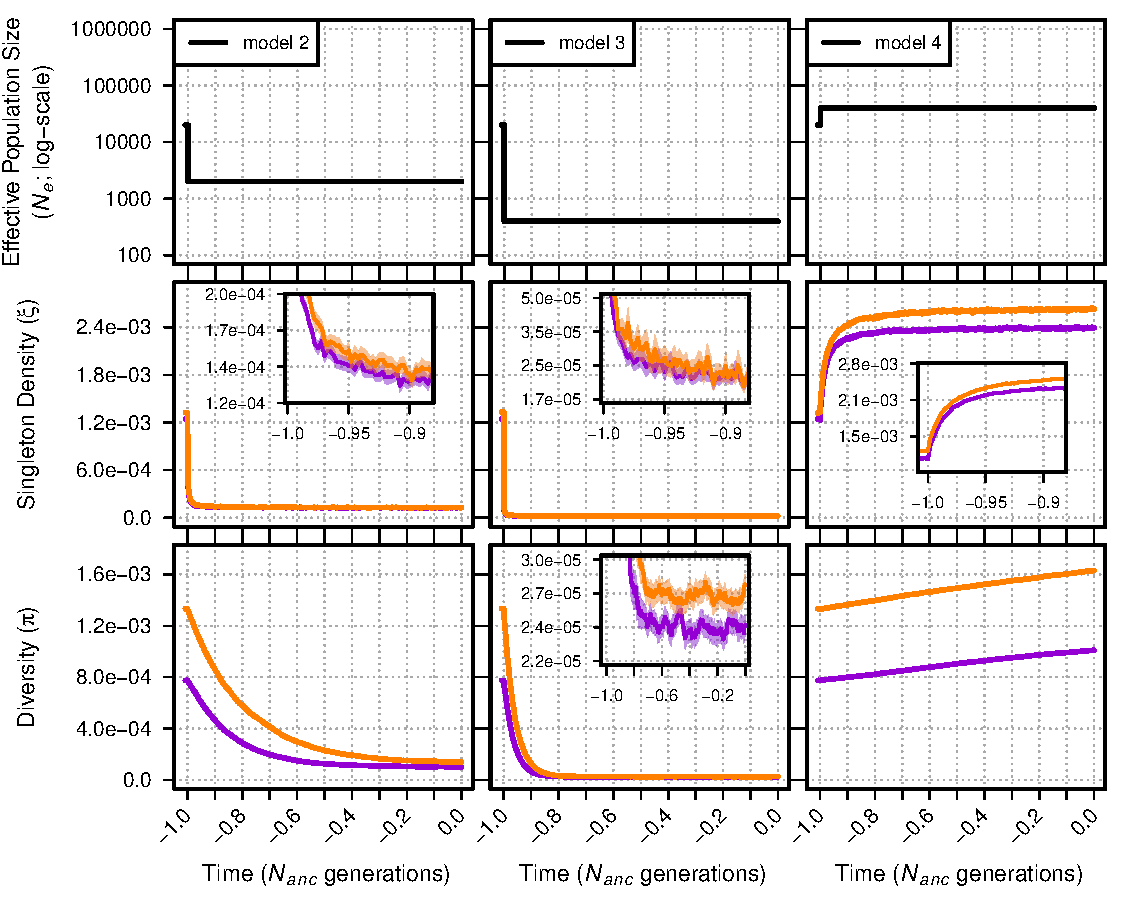
\includegraphics[width=\linewidth]{figures/FigS6_new.pdf}
\caption{Singleton density ($\xi$ per site) and diversity ($\pi$ per site) for models 2-4.
The top panel shows each demographic model; time proceeds forward from left to right and is scaled by the $N_e$ of the population at the initial generation ($N_{anc}$; 20,000 individuals).
Diverstiy statistics are shown for neutral simulations (orange lines) and simulations with BGS (violet lines).
Insets show diversity using a log scale for improved detail.
Envelopes are 95\% CIs calculated from 10,000 bootstraps of the original simulation data.}
\label{fig:S6}
\end{figure}

To examine the interaction of demography and selection observed in empirical data \citep{beissinger2016recent,torres2018human}, we normalize $\pi$ and $\xi$ in models of BGS by their equivalent statistics generated under the same demographic model in the absence of any selection ($\pi_0$ and $\xi_0$).
We observed that $\pi/\pi_0$ and $\xi/\xi_0$ were dynamic through time in response to demography, with changes occurring to both their magnitude and direction (Figure \ref{fig:1}).
Moreover, changes to $\xi/\xi_0$ occurred more rapidly through time compared to $\pi/\pi_0$.
For example, in model 2 we observed a dip and rise in the $\xi/\xi_0$ statistic relative to equilibrium (model 1) within the first $\approx 0.1N_{anc}$ generations ($N_{anc}$ refers to the $N_e$ of the ancestral population prior to any demographic change).
Yet, for the same model, $\pi/\pi_0$ remained depressed for over 0.5 $N_{anc}$ generations (Figure \ref{fig:1}).
Similar patterns were observed for model 3, which experienced a greater reduction in size, although the pattern is less clear because of the greater sampling variance of $\xi/\xi_0$ due to the overall lower number of singletons.
In both population contraction models  $\pi/\pi_0$ and $\xi/\xi_0$ appeared to plateau at levels above that of model the equilibrium model.
In contrast, we observed markedly different dynamics in our model of a simple population expansion (model 4), with a sustained increase in $\pi/\pi_0$ but only a transient increase in $\xi/\xi_0$ within the first $\approx 0.1N_{anc}$, followed by a reduction in $\xi/\xi_0$ to levels below that of the equilibrium model.

\begin{figure}[]
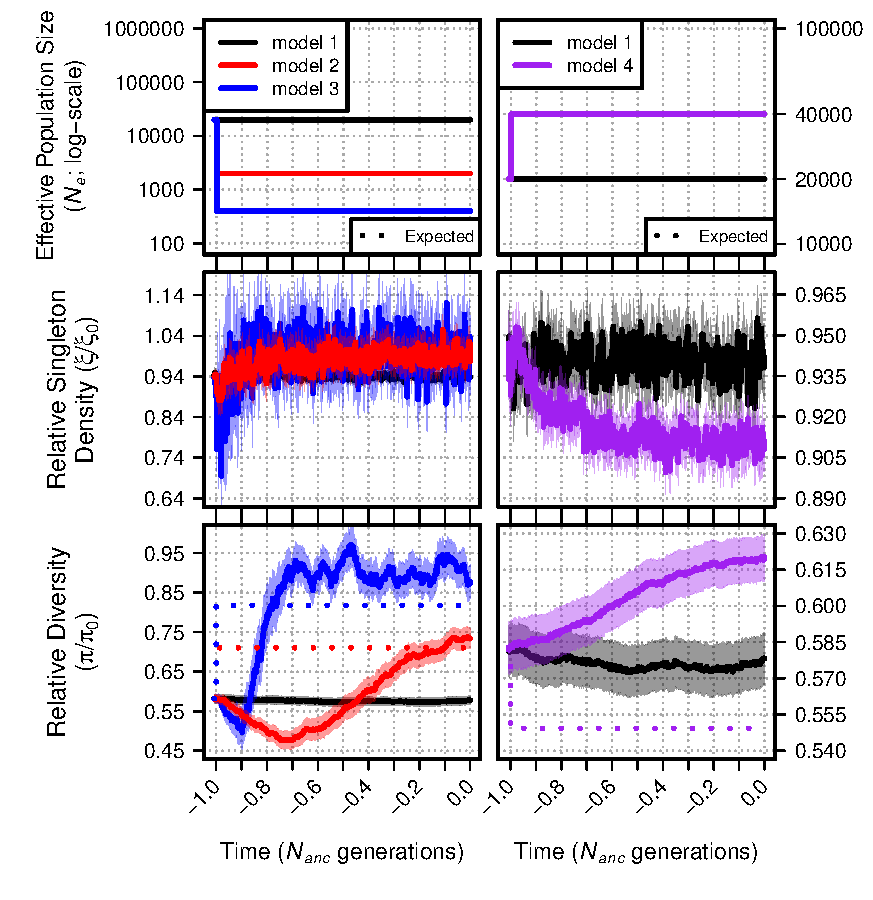
\includegraphics[width=\linewidth]{figures/F1newclean_2.pdf}
\caption{Relative singleton density ($\xi/\xi_0$) and relative diversity ($\pi/\pi_0$) across time for demographic models 1-4.
The top panel shows each demographic model as in Figure \ref{fig:S6}.
Black lines show $\xi/\xi_0$ and $\pi/\pi_0$ from simulations of a constant sized population (model 1).
Dotted lines in the bottom panel show the equilibrium  expectation of $\pi/\pi_0$ from  \citet{nordborg1996effect} given the specific selection parameters and the instantaneous $N_e$ at each time point.
Envelopes are 95\% CIs calculated from 10,000 bootstraps of the original simulation data.}
\label{fig:1}
\end{figure}

Changes in population size should lead to changes in the rate of genetic drift and the efficacy of natural selection and, thus, changes in the magnitude of BGS over time.
Indeed, under equilibrium conditions (and if mutations that are effectively neutral can be ignored) the classic model of BGS \citep{nordborg1996effect} predicts weaker BGS (with higher $\pi/\pi_0$) for smaller populations and stronger BGS (with lower $\pi/\pi_0$) for larger populations.
To compare these predictions to those of our simple demographic models, we calculated the predicted equilibrium $\pi/\pi_0$ under the classic model given the instantaneous $N_e$ at each generation.
In all three simple demographic models we observed that changes in $\pi/\pi_0$ over the short term differed qualitatively from the classic model  (Figure \ref{fig:1}; bottom panel).
The classic model predicts a higher value for $\pi/\pi_0$ in a smaller population, yet we observed a transient drop in $\pi/\pi_0$ directly after a contraction (models 2 and 3).
Similarly, while the classic model predicts a decrease in $\pi/\pi_0$ in larger populations, we observed an increase in $\pi/\pi_0$ with a population expansion (model 4).
The trajectory of $\pi/\pi_0$ changed in our bottleneck models, eventually approaching the expectation predicted by the classic model, while $\pi/\pi_0$ in the expansion model continued to increase over the entire course of the simulation.

\subsection{Background selection under bottleneck-expansion models}

We built upon the simple two epoch demographic models to test more complex scenarios and better understand the relative effects of different events on patterns of diversity under BGS.
Specifically, we simulated a population undergoing a contraction similar in size to models 2 and 3, but with a subsequent expansion to 400,000 individuals by the final generation (Figure \ref{fig:models2}).
These bottleneck-expansion models included both ancient (1.0 $N_{anc}$ generations in the past; models 5-8) and recent (0.1 $N_{anc}$ generations in the past; models 9-12) bottlenecks with either an instantaneous expansion (models 5-6, 9-10) or a sustained bottleneck (models 7-8, 11-12).
These models recapitulated several patterns observed in our simple bottleneck models, but with added dynamics.
In all cases, diversity  in models with BGS was both lower (Figures \ref{fig:S4}-\ref{fig:S5}) and changed more rapidly (Figures \ref{fig:S7}-\ref{fig:S8}) than in neutral simulations.
Changes in diversity also occurred more quickly in models with a stronger or sustained bottleneck, and  $\xi$ again exhibited more rapid dynamics than did $\pi$.
Mirroring results from our simple bottleneck scenarios, models with an ancient bottleneck (models 5-8) showed a transient decrease in $\xi/\xi_0$ and $\pi/\pi_0$ followed by an increase to higher values (Figure \ref{fig:3new}).
Again changes in $\pi/\pi_0$ contrast with the expectations of the classic model, where  BGS is expected to become more efficient in larger populations, thus resulting in an expected decrease in $\pi/\pi_0$ through time (Figure \ref{fig:3new}, dotted line).
But while both $\pi/\pi_0$ and $\xi/\xi_0$ remain elevated in our simple bottleneck models, $\xi/\xi_0$ in the bottleneck-expansion models shifts direction during the course of the expansion and begins to decline, eventually reaching values below that of the equilibrium population.
Though the trajectories of $\pi/\pi_0$ and $\xi/\xi_0$ were truncated for models in which the bottleneck occurred in the recent  past (models 9-12; 0.1 $N_{anc}$ generations), they nonetheless appeared to behave qualitatively similar to ancient bottleneck models (Figure \ref{fig:S912}). Notably, for these models, the ending values of $\xi/\xi_0$ and $\pi/\pi_0$ were in the opposite direction relative to model 1 when compared to the models with longer demographic histories.

\begin{figure}[t!]
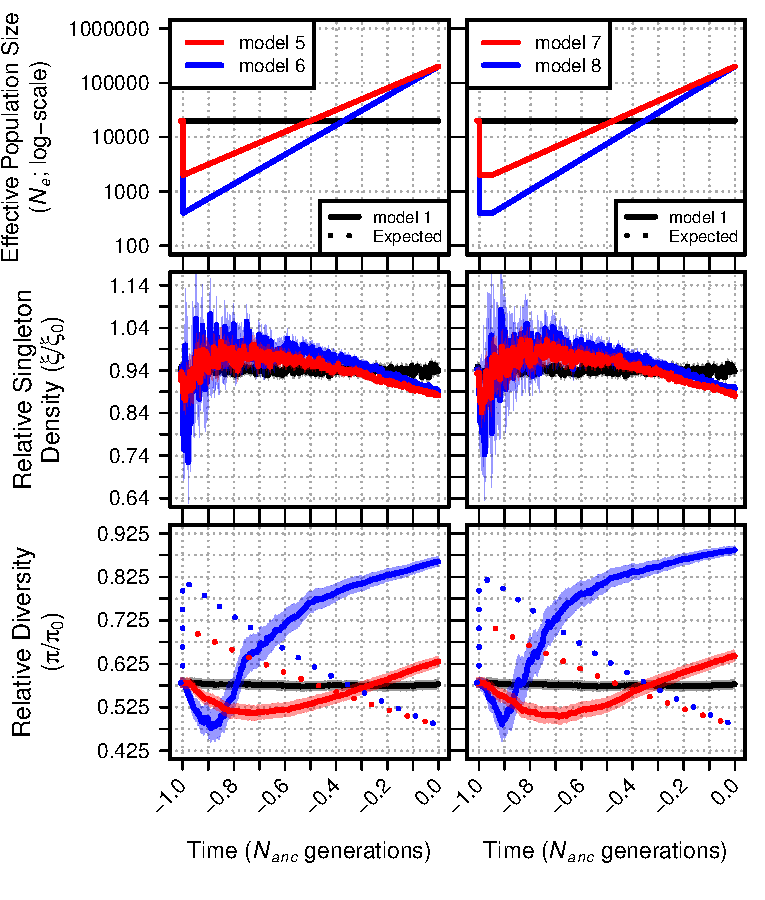
\includegraphics[width=\linewidth]{figures/fig3newclean.pdf}
\caption{Relative singleton density ($\xi/\xi_0$) and relative diversity ($\pi/\pi_0$) across time for demographic models 1 and 5-8.
The top panel shows each demographic model; time proceeds forward from left to right and is scaled by the $N_e$ of the population at the initial generation ($N_{anc}$; 20,000 individuals).
Black lines show $\xi/\xi_0$ and $\pi/\pi_0$ from simulations of a constant sized population (model 1).
Dotted lines in the bottom panel show the equilibrium expectation of $\pi/\pi_0$ from  \citet{nordborg1996effect} given the specific selection parameters and the instantaneous $N_e$ at each time point.
Envelopes are 95\% CIs calculated from 10,000 bootstraps of the original simulation data.}
\label{fig:3new}
\end{figure}

\subsection{Patterns of diversity across the 200 kb neutral region}

We also measured patterns of $\pi/\pi_0$ across time for the entire 200 kb neutral region.
Doing so showed the characteristic ``trough'' structure of increasing relative diversity as a function of genetic distance from the deleterious locus (model 5 shown in Figure \ref{fig:200kb}, see Figure \ref{fig:all200} for all models). Change in $\pi/\pi_0$ over time generally followed patterns observed in the neutral window closest to the selected region. In all of our ancient bottleneck models (models 2-3, 5-8), for example, we see a decline in $\pi/\pi_0$ across the entire region followed by an increase to levels higher than in the ancestral population. For recent bottlenecks (models 9-12) we see a consistent decline with no recovery and in our simple expansion model (model 4) $\pi/\pi_0$ increases monotonically through time.

Yet, these general patterns obscure more subtle changes in the slope of $\pi/\pi_0$ with increasing distance from the selected region. In models with a stronger bottleneck (models 3, 6 and 8), where we expect the efficacy of selection to be most affected, we see that the slope $\pi/\pi_0$ flattens over time, completely erasing the trough of diversity in the most extreme case without a recovery (model 3). 


\begin{figure}[t!]
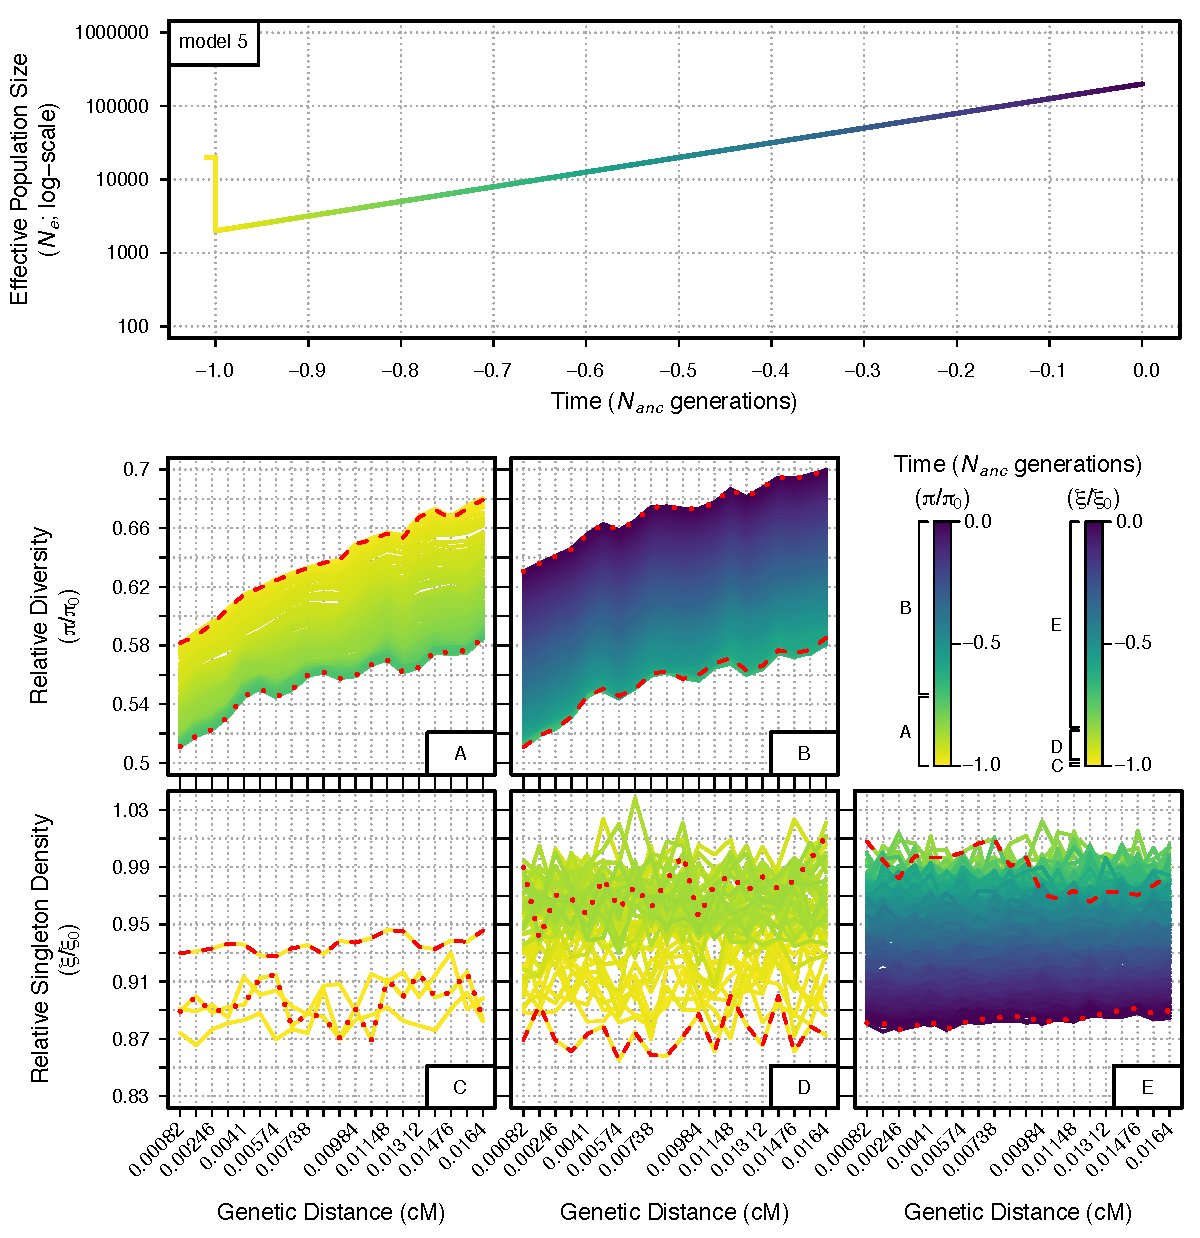
\includegraphics[width=\linewidth]{figures/FigS13.pdf}
\caption{Temporal and spatial dynamics of relative diversity ($\pi/\pi_0$) and singleton density ($\xi/\xi_0$) under demographic model 5 across a neutral 200 kb region. The genetic distance of each 10 kb bin from the selected locus is indicated on the x-axis of the bottom panels. Each line measuring $\pi/\pi_0$ and $\xi/\xi_0$ in the bottom panels represent one of the 401 discrete generations sampled from the demographic model; colors follow the demographic model in the top panel (time is scaled as in Figures \ref{fig:S6}-\ref{fig:3new}) and in the figure legend. Multiple plots are given in order to prevent overlap of the measurements between generations (see legend for specific generations covered in each plot). Red dashed lines and red dotted lines indicate the first and last generation measured within each plot (respectively).}
\label{fig:200kb}
\end{figure}

Finally, while $\xi/\xi_0$ across the region largely followed patterns seen in the neutral window most proximal to the selected locus, a closer look across the 200 kb regions of most models yielded no clear patterns. 
Troughs were slightly apparent for the final generations of some models (models 5 and 7), but the stochasticity among 10 kb windows for $\xi/\xi_0$ swamped any other patterns that might otherwise be evident.

%%%%%%%%%%%%%%%%%%%%%%%%%%%%%%%%%%%%%%%%%%%%%%%%%%%%%%
\section{Discussion}
%%%%%%%%%%%%%%%%%%%%%%%%%%%%%%%%%%%%%%%%%%%%%%%%%%%%%%

\subsection{General patterns of diversity}

A long history of both theoretical \citex{} and empirical \citex{} population genetics work has provided a clear picture of the impacts of demographic change on neutral sites in the absence of linked selection.
We know, for example, the impact of simple bottleneck and growth models such as those simulated here on the allele frequency spectrum \citex{}.
Theory also offers clear direction on the long-term effects of decreases in effective population size on the efficacy of natural selection \citex{}.
Likewise, now classic theory on background selection provides a solid theoretical expectation for the effects of linked selection on diversity in populations at demographic equilibrium \citep{nordborg1996effect}.

Despite these efforts, there are no formal theoretical treatments describing expected patterns of the interaction of demography and linked selection, and only one limited simulation attempts \citex{comeron2017background}.
Notably, there remains substantial confusion in empirical population genetic analyses, where authors often equate long-term predictions of changes in effective populations size on the efficacy of natural selection to short-term responses under non-equilibrium demography.
Here, we use exhaustive simulations and analysis of different demographic models with and without background selection to show that predictions from such equilibrium models generally fail to hold up over shorter time scales, and that the predicted impacts of the combined effects of demography and linked selection depend strongly on the details of the demographic model as well as the timing of sampling.

In each of our models, the initial effects observed are dominated by demography alone, and fit well with theoretical expectations.
Loss of diversity in the first few generations occurs equally across the entire region, independent of the distance from the selected region.
While equilibrium models predict that the effects of BGS should be attenuated in populations with lower $N_e$ due to the decreased efficacy of purifying selection, we instead observed a drop in $\pi/\pi_0$  after the bottleneck, and a greater loss in models with a stronger bottleneck \jri{cite some figs}, demonstrating that the populations were dominated by the effects of allelic loss.
These observations make it clear that effects of BGS on $\pi/\pi_0$ immediately following a reduction in $N_e$ were not driven by a change in the efficacy of natural selection from population decline, but rather by allelic loss within these regions.
Similarly, while theory predicts a decrease in $\pi/\pi_0$ in expanding populations, we see the initial response is instead an increase\jri{cite figs}.

Although the initial changes in diversity are dominated by the impacts of demography, as population size shifts the efficacy of natural selection begins to change as well.
In our simple bottleneck models, for example,  $\pi/\pi_0$ stops declining and begins to increase, eventually reaching higher values as expected under equilibrium \jri{cite figures}.
This change reflects the inability of a smaller population to effectively select against new deleterious mutations, rendinerg such alleles effectively neutral \jri{refs}.
These effects are presumably why we see the rate of increase of $\pi/\pi_0$ slow and eventually plateau in models incorporating both bottlenecks and growth \jri{figures}.
Changes in the efficacy of selection are also readily observed in comparisons of diversity across neutral windows varying in recombination distance from the selected region \jri{cite figures}.
Diversity in the ancestral population increases with  distance from the selected regions as expected under classical models of BGS at equilibrium \citex{}. 
But while the slope of this relationship remains constant in the generations initially following population size change in our simple bottleneck models, it begins to flatten as the lower effective population size changes in the efficacy of natural selection cause the slope to flatten  \jri{cite fig}.
%\jri{where do we discuss fact they don't perfectly hit equilibrium expectations, and that this may be because of our $\gamma$ threshold}
\jri{can we connect the inflection points of change in Ne? can we say e.g. that the inflection point happens after $N_{bottleneck}$ gens, then we see increase?}
%1) time 2) However, we note that this expectation underestimated $\pi/\pi_0$ for model 3 because the threshold of $s < 0.15/2N_e$ was likely not conservative enough to ignore deleterious mutations that behave neutrally under the low $N_e$ size of 400 for that model.

The diversity-reducing effects of BGS have often been modeled as a reduction in $N_e$ \citep{charlesworth1993effect}, though we caution that effects of BGS on the SFS cannot be simplified to this extent \citep{cvijovic2018effect}.
Like a reduction in $N_e$, however, BGS exacerbates the stochastic process of drift.
And because the relevant timescale for allele frequency evolution is scaled by the rate of drift \citex{}, both the reduction and recovery of $\pi/\pi_0$ to equilibrium levels happen over fewer generations in populations with stronger bottlenecks and in regions impacted by BGS.
We see this borne out in comparisons of models with stronger \jri{figure} or more sustained \jri{figure} bottlenecks, as well as comparisons of models with BGS to their equivalent neutral scenarios \jfir{figure}.
%For example, the inflection point at which $\pi$ under BGS surpassed $\pi$ under neutrality occurred at -0.305 and -0.848 $N_{anc}$ generations for models 7 and 8, respectively (Figure S7). For models 5 and 6, these inflection points occurred later in time at -0.235 and -0.785 $N_{anc}$ generations, respectively. Further, the final $\pi/\pi_0$ values for models 7 and 8 were 0.643 and 0.887 but for models 5 and 6, they were only 0.631 and 0.860. Thus, the sustained lower $N_e$ of models 7 and 8 aided in accelerating the approach to the new equilibrium established by population reduction. 
This framework also helps explain the slow changes observed in expanding populations , as increases in the effective size attenuate the rate of drift.

Because singleton variants represent very recent mutations, changes in $\xi/\xi_0$ responded quickly to changes in $N_e$.  
In our simple expansion model, for example, while $\pi/\pi_0$ never stops increasing, we see a relatively rapid increase in $\xi/\xi_0$, followed by a decrease as a larger population size increases the efficacy of selection against new deleterious mutants. 
And while theoretical predictions for $\xi/\xi_0$ are not straightforward, singleton diversity in the simple expansion model quickly plateaus at a new value below that of the ancestral population, consistent with having reached a new equilibrium value.
However, signals using rare frequency bins such as $\xi$ are inherently more difficult to capture, partly because it is less affected than $\pi$ since BGS perturbs common frequency bins of the SFS more than rare ones \citep{cvijovic2018effect}.
In addition, we observe much higher variance  for $\xi/\xi_0$ compared to $\pi/\pi_0$ due to the smaller number of sites contributing to $\xi$. 

Overall, then, we find that theoretical models of population demographic change or selection alone are insufficient to predict changes in diversity when both processes are at play. 
Both $\pi/\pi_0$ and $\xi/\xi_0$ show initial changes that often conflict with predictions from equilibrium models of BGS, reflecting instead the effects of rapid demographic change.
But the rate at which diversity patterns begin to exhibit the impact changes in the efficacy of natural selection varies, differing between $\pi/\pi_0$ and $\xi/\xi_0$ and depending on the effects of demography and BGS on the rate of drift and thus the timescale over which changes can be observed.
Although we have simulated under a mixture distribution of selection coefficients for new mutations (see Methods), this distribution will also play an important role in determining the threshold above which new mutations are efficiently removed by selection.
In practice, it will be difficult to know any of these features in empirical data, and thus simple predictions --- for example that a bottleneck will reduce the efficacy of natural selection and lead to increases in $\pi/\pi_0$ --- are likely to be difficult to make with much accuracy.

\subsection{Comparisons to empirical data}

One of the motivations for the work presented here is the fact that empirical analyses evaluating the impact of demography on linked selection have come to conflicting conclusions \citep{torres2018human, beissinger2016recent}.
Cultivated maize, for example, is thought to have undergone a bottleneck during the process of domestication \citep{eyre1998investigation,tenaillon2004selection,wright2005effects}, followed by a substantial expansion to a modern size several orders of magnitude larger than its wild ancestor teosinte \citep{beissinger2016recent, bellon2018evolutionary}.
A recent analysis of selection at linked sites in  maize and teosinte found differences, and interpreted them to be due to the timing of these demographic events.
\citet{beissinger2016recent} found that $\pi/\pi_0$ exhibited a greater trough around selected sites in teosinte, consistent with this taxon's larger long-term $N_e$.
However, their analysis of $\xi/\xi_0$ found the opposite pattern --- stronger effects in maize than teosinte --- a result the authors interpreted as a reflection of the post-domestication expansion and increased efficacy of selection in maize in the recent past.

Human demographic history appears at least qualitatively similar to that of maize, with a bottleneck associated with migration out of Africa followed by considerable recent population expansion \citep{tennessen2012evolution}.
In spite of this, however, analysis of selection at linked sites in humans produced different results \citep{torres2018human}.
The bottlenecked non-African populations were found to have lower $\pi/\pi_0$ but higher $\xi/\xi_0$ than African populations. The authors interpreted this as the effects of a demographic bottleneck being exacerbated in regions of BGS, leading to greater losses of diversity ($\pi$) in Europeans. However, the authors also concluded that the lowered $N_e$ resulting from the European bottleneck led to weaker effects of BGS overall, which were manifested in the higher observed values of $\xi/\xi_0$.

While there are a number of challenges associated with accurate estimation of historical demography in natural and domesticated populations \citex{}, our models highlight the fact that results seen in both maize and humans are plausible under even relatively simple models that are broadly consistent with the dynamics of these two systems.
For example, under the bottleneck-expansion models of Figure \ref{fig:3new}, sampling in the present (generation 0) returns results similar to those seen in maize, with $\pi/\pi_0$ higher than a constant-size reference population but $\xi/\xi_0$ showing lower values due to the increased efficacy of selection in the expanding population.
Yet, if a sample was taken $\approx -0.8N_{anc}$ - $-0.6N_{anc}$ generations in the past for model 5 or 7, they would reveal the observed pattern in humans, with a lower $\pi/\pi_0$ but a higher $\xi/\xi_0$, reflecting the impacts of a recent bottleneck. Indeed, in our simulations of demographic models with a short time span (models 9-12), we also observe these results when sampling in the present (Figure \ref{fig:S912}).

\section{Conclusions}

Genetic diversity across the genome is determined by the complex interplay of mutation, demographic history, and the effects of both direct and linked natural selection. 
While each of these processes is understood to a degree on its own, in many cases we lack either theory or sufficient empirical data to capture the effects of their interaction.

Linked selection, in particular, is increasingly recognized as perhaps the primary determinant of patterns of diversity along a chromosome, but our ability to infer its impact is often complicated by changes in population size.
Indeed, many authors make the simplifying assumption that linked selection in such non-equilibrium populations can be effectively modeled using classic theory and simply scaling the  effective population size $N_e$.
Our extensive simulations show that this is not the case.

We find that the relationship between linked selection and demographic change is complex, with short-term dynamics often qualitatively different from predictions under classic models.
These results suggest that inferring the impact of population size change on linked selection should be undertaken with caution, and is only really possible with a thorough understanding of the demographic history of the populations of interest.

\section{Acknowledgments}

MGS and JR-I would like to acknowledge funding from NSF Plant Genome Grant 1238014.
We would also like to thank Felix Andrews for statistical advice, although we did not follow it.

\bibliography{example-bibliography}

%\pagebreak
\onecolumn

\beginsupplement
\section*{Supplement}

\begin{sidewaystable}
\begin{tabular}{ | l | c | c | c | c | c | c | c | c | c | c | c | c | }
\hline
	\textbf{parameter} & \textbf{model 1} & \textbf{model 2} & \textbf{model 3} & \textbf{model 4} & \textbf{model 5} & \textbf{model 6} & \textbf{model 7} & \textbf{model 8} & \textbf{model 9} & \textbf{model 10} & \textbf{model 11} & \textbf{model 12} \\ \hline
	ancestral population size ($N_e$ [$N_{anc}$]) & 20000 & 20000 & 20000 & 20000 & 20000 & 20000 & 20000 & 20000 & 20000 & 20000 & 20000 & 20000 \\ \hline
	bottleneck/expansion population size ($N_e$) & NA & 2000 & 400 & 40000 & 2000 & 400 & 2000 & 400 & 2000 & 400 & 2000 & 400 \\ \hline
	bottleneck time length ($N_{anc}$ generations) & NA & 1 & 1 & NA & 0 & 0 & 0.05 & 0.05 & 0 & 0 & 0.05 & 0.05 \\ \hline
	expansion time length ($N_{anc}$ generations)* & NA & NA & NA & 1 & 1 & 1 & 0.95 & 0.95 & 0.1 & 0.1 & 0.05 & 0.05 \\ \hline
	final population size ($N_e$) & 20000 & 2000 & 400 & 40000 & 200000 & 200000 & 200000 & 200000 & 200000 & 200000 & 200000 & 200000 \\ \hline
    \multicolumn{13}{l}{*note that the population expansions of models 5-12 are exponential growth models and that model 4 is an instantaneous growth model}
\end{tabular}

\caption{Demographic parameters for models 1-12}
\label{table:params}
\end{sidewaystable}
\pagebreak

\begin{figure*}[h!]
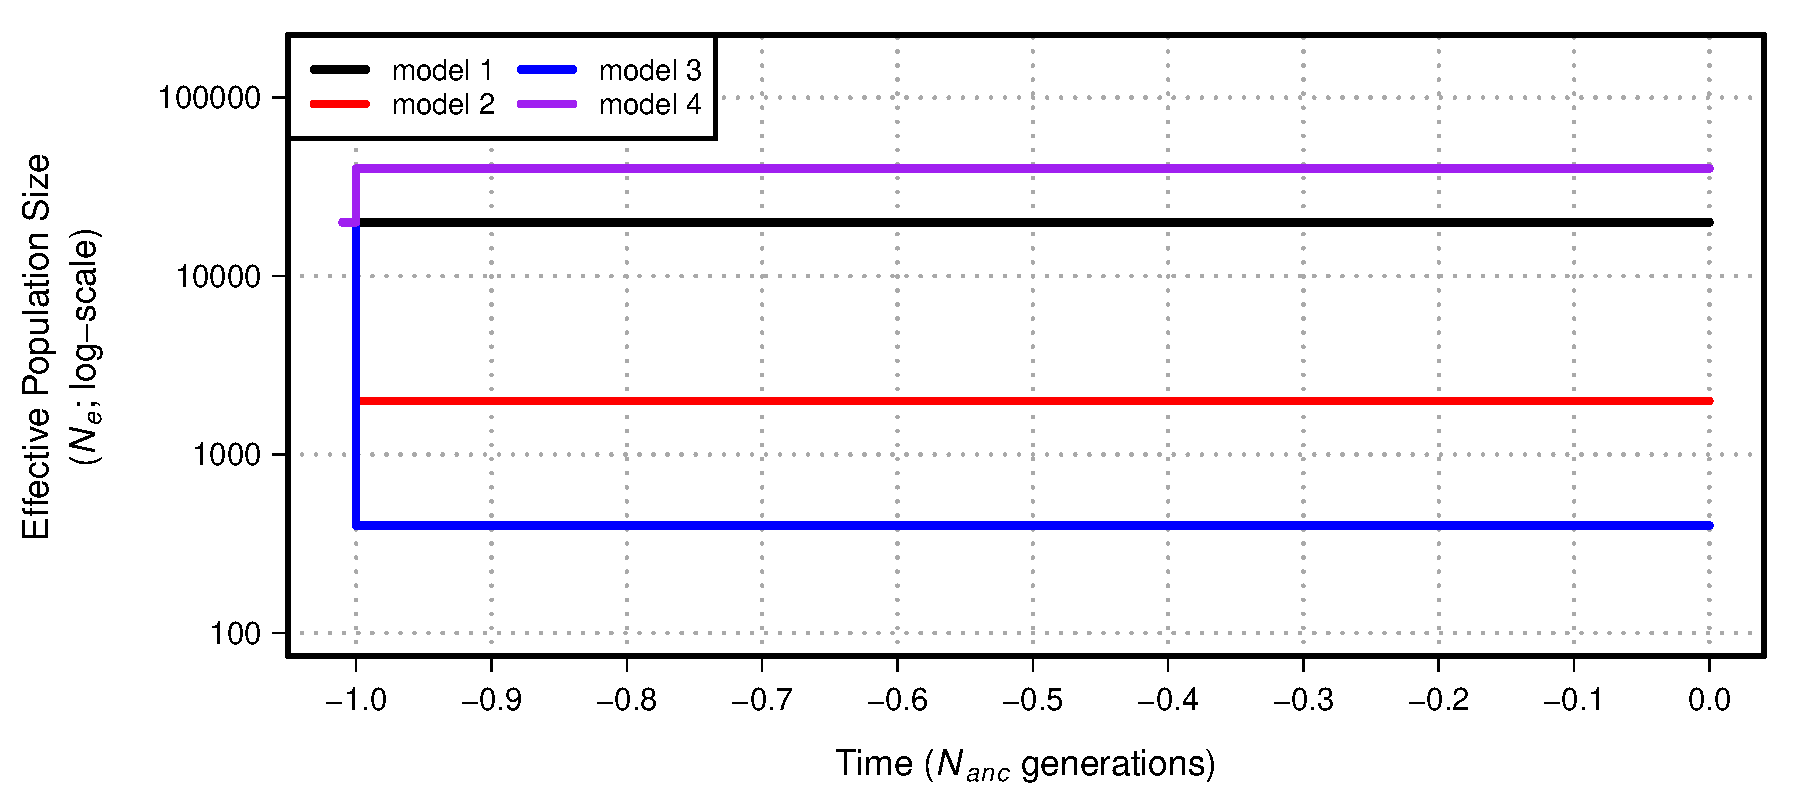
\includegraphics[width=0.8\linewidth]{figures/FigS1.pdf}
\caption{Demographic models 1-4 simulated in our study.
Time proceeds forward from left to right and is scaled by the $N_e$ of the population at the initial generation ($N_{anc}$; 20,000 individuals).
Demographic model 2 experiences a population contraction to 2000 individuals while demographic model 3 experiences a population contraction to 400 individuals.
Demographic model 4 experiences a population expansion to 40,000 individuals.
All population size changes are instantaneous for models 2-4.
See Table \ref{table:params} for additional model parameters.}
\label{fig:models1}
\end{figure*}
\pagebreak

\begin{figure*}[t]
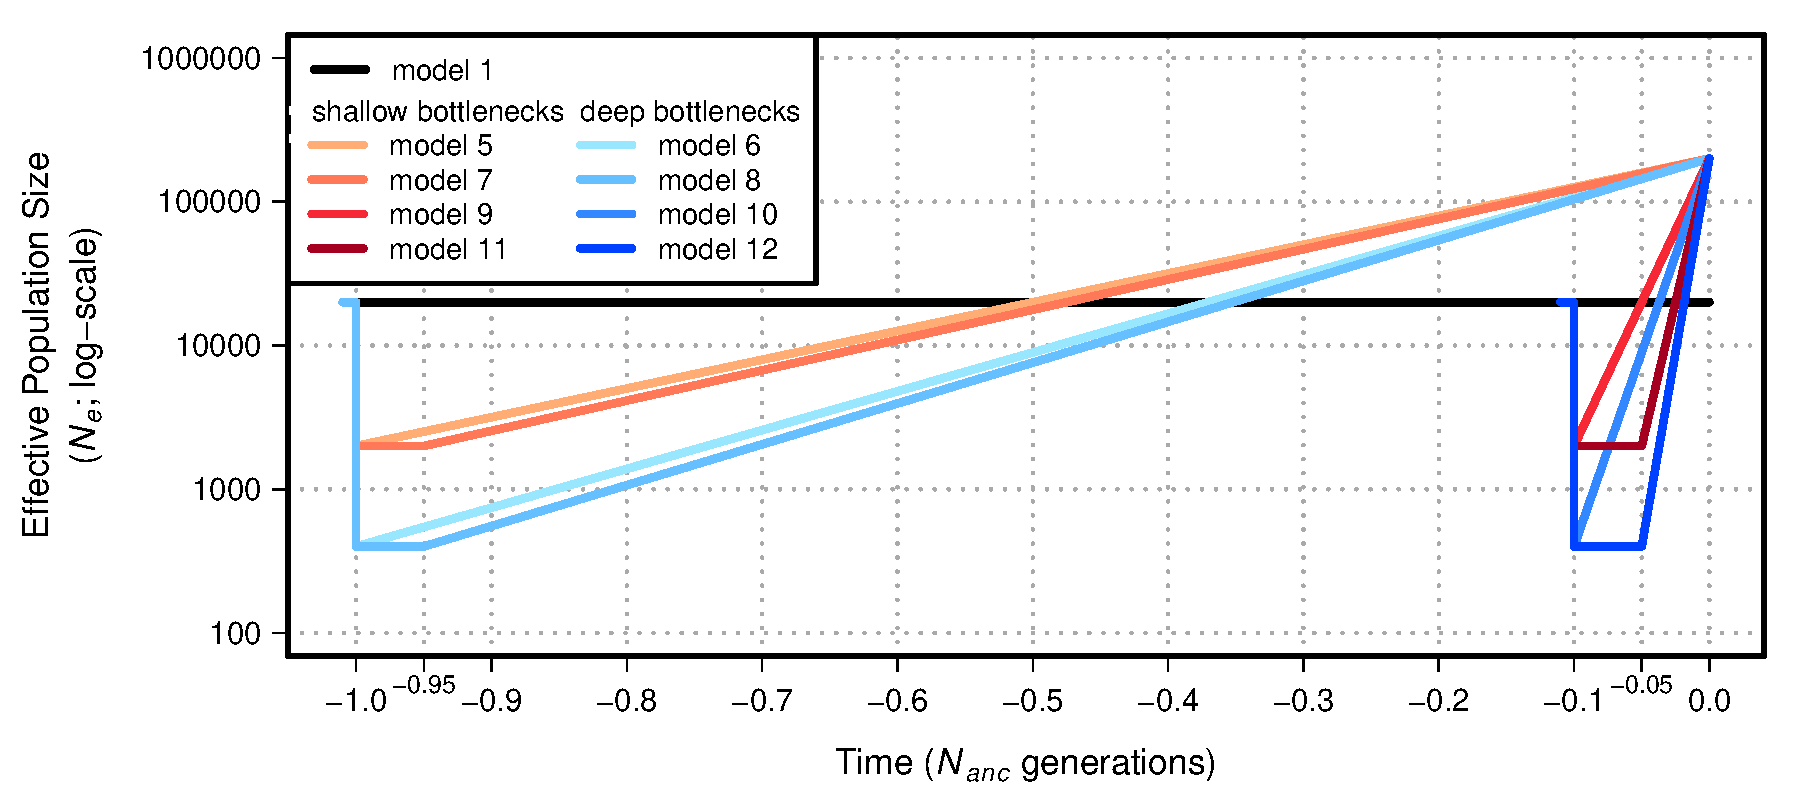
\includegraphics[width=0.8\linewidth]{figures/FigS2.pdf}
\caption{Demographic models 1 and 5-12 simulated in our study.
Time proceeds forward from left to right and is scaled by the $N_e$ of the population at the initial generation ($N_{anc}$; 20,000 individuals).
Demographic models with a shallow bottleneck (models 5, 7, 9, and 11) experience a population contraction to 2000 individuals while demographic models with a deep bottleneck (models 6, 8, 10, and 12) experience a population contraction to 400 individuals.
After contraction, demographic models 5-12 undergo exponential growth to a final population size of 200,000 individuals.
See Table \ref{table:params} for additional model parameters.}
\label{fig:models2}
\end{figure*}
\pagebreak

\begin{figure*}[t]
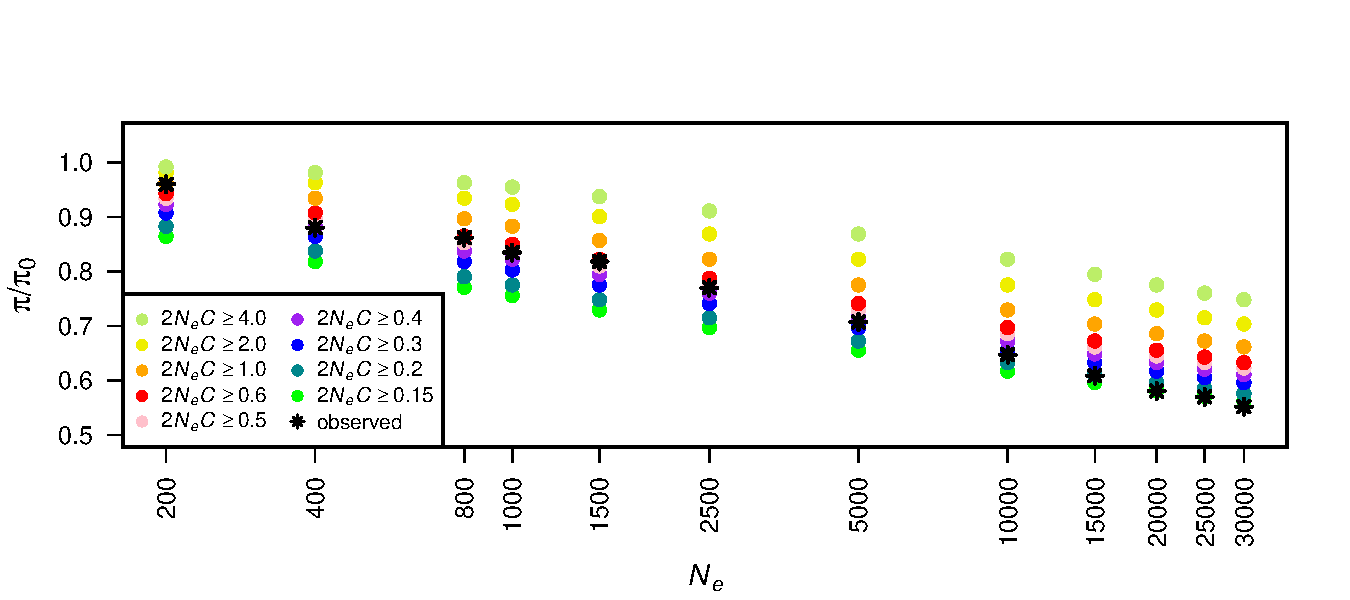
\includegraphics[width=.9\linewidth]{figures/FigS21.pdf}
\caption{Estimate of $\pi/\pi_0$ from the classic model \citep{nordborg1996effect} across different population sizes and different truncation thresholds on selection.
Different $\gamma$ values used to truncate selection ($C$) for the classic model are shown in the legend ($2N_eC \geq \gamma$).
Black stars represent the observed $\pi/\pi_0$ from running simulations of BGS.}
\label{fig:nordborgsims}
\end{figure*}
\pagebreak

\begin{figure*}[t]
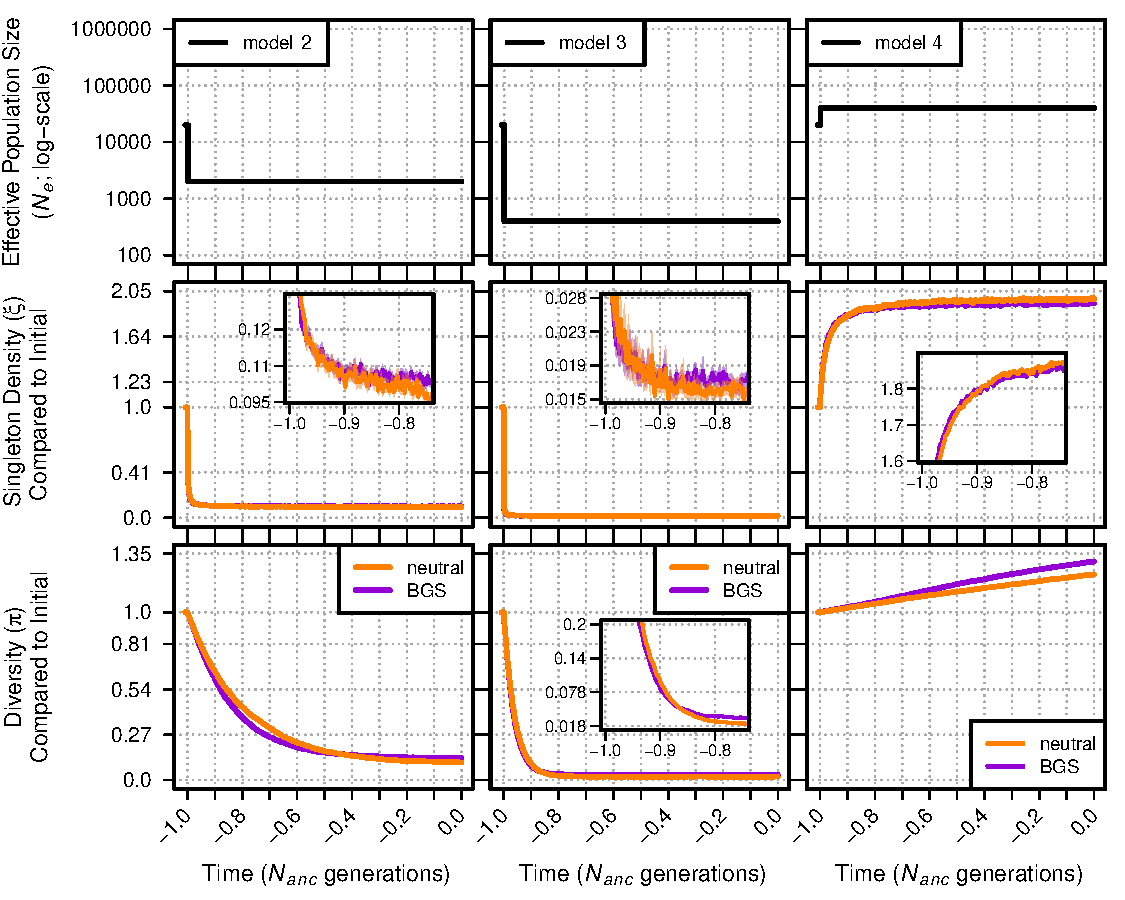
\includegraphics[width=.9\linewidth]{figures/FigS9.pdf}
\caption{Singleton density ($\xi$) and diversity ($\pi$) for demographic models 2-4 under neutrality (orange lines) and BGS (violet lines) relative to their values in the initial generation prior to demographic change.
The top panel shows each demographic model as in Figure \ref{fig:S6}.
For greater detail, insets show data for generations over a smaller time scale and smaller y-axis (note: y-axes for insets are scaled linearly).
Envelopes are 95\% CIs calculated from 10,000 bootstraps of the original simulation data.
The data used for this figure is identical to that of Figure \ref{fig:S6}.}
\label{fig:S9}
\end{figure*}
\pagebreak

\begin{figure}[t]
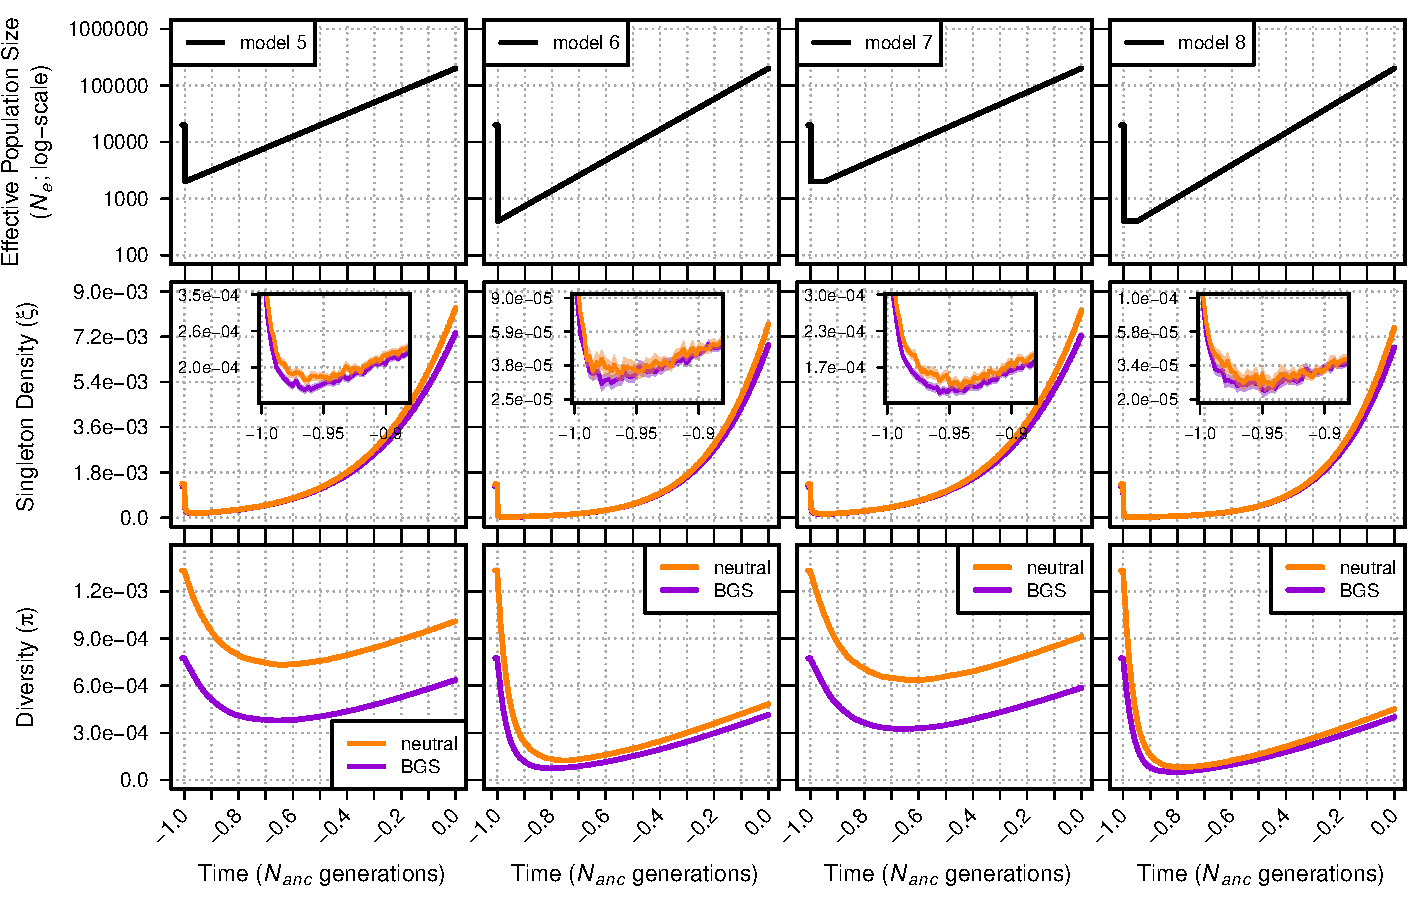
\includegraphics[width=\linewidth]{figures/FigS4.pdf}
\caption{Singleton density ($\xi$ per site) and diversity ($\pi$ per site) for models 5-8.
The top panel shows each demographic model; time proceeds forward from left to right and is scaled by the $N_e$ of the population at the initial generation ($N_{anc}$; 20,000 individuals).
Diversity statistics are shown for neutral simulations (orange lines) and simulations with BGS (violet lines).
Insets show diversity using a log scale for improved detail.
Envelopes are 95\% CIs calculated from 10,000 bootstraps of the original simulation data.}
\label{fig:S4}
\end{figure}
\pagebreak

\begin{figure}[t]
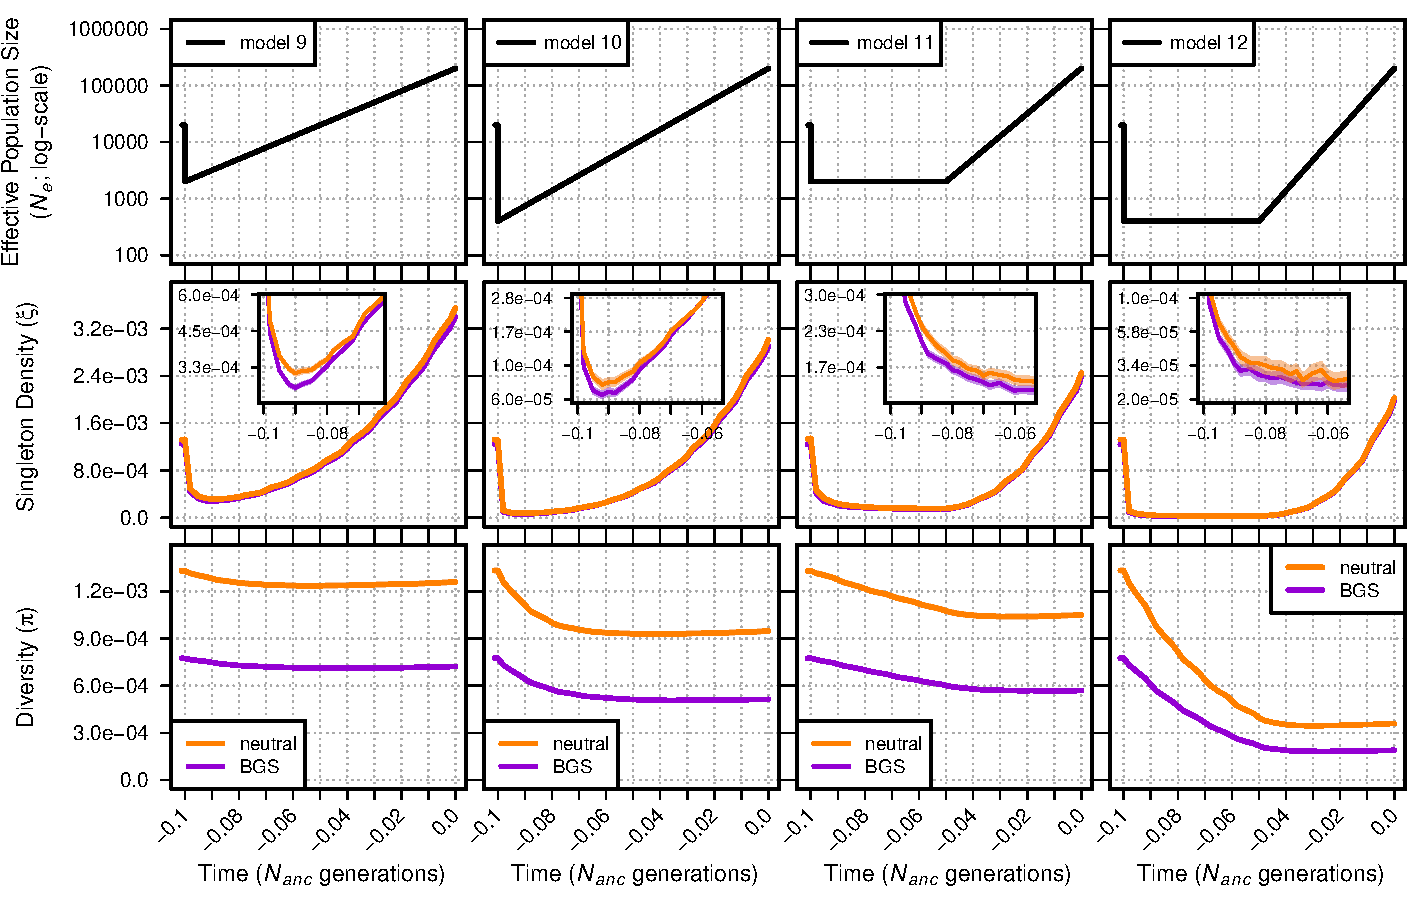
\includegraphics[width=\linewidth]{figures/FigS5.pdf}
\caption{Singleton density ($\xi$ per site) and diversity ($\pi$ per site) for models 9-12.
The top panel shows each demographic model; time proceeds forward from left to right and is scaled by the $N_e$ of the population at the initial generation ($N_{anc}$; 20,000 individuals).
Diversity statistics are shown for neutral simulations (orange lines) and simulations with BGS (violet lines).
Insets show diversity using a log scale for improved detail.
Envelopes are 95\% CIs calculated from 10,000 bootstraps of the original simulation data.}
\label{fig:S5}
\end{figure}
\pagebreak

\begin{figure*}[h!]
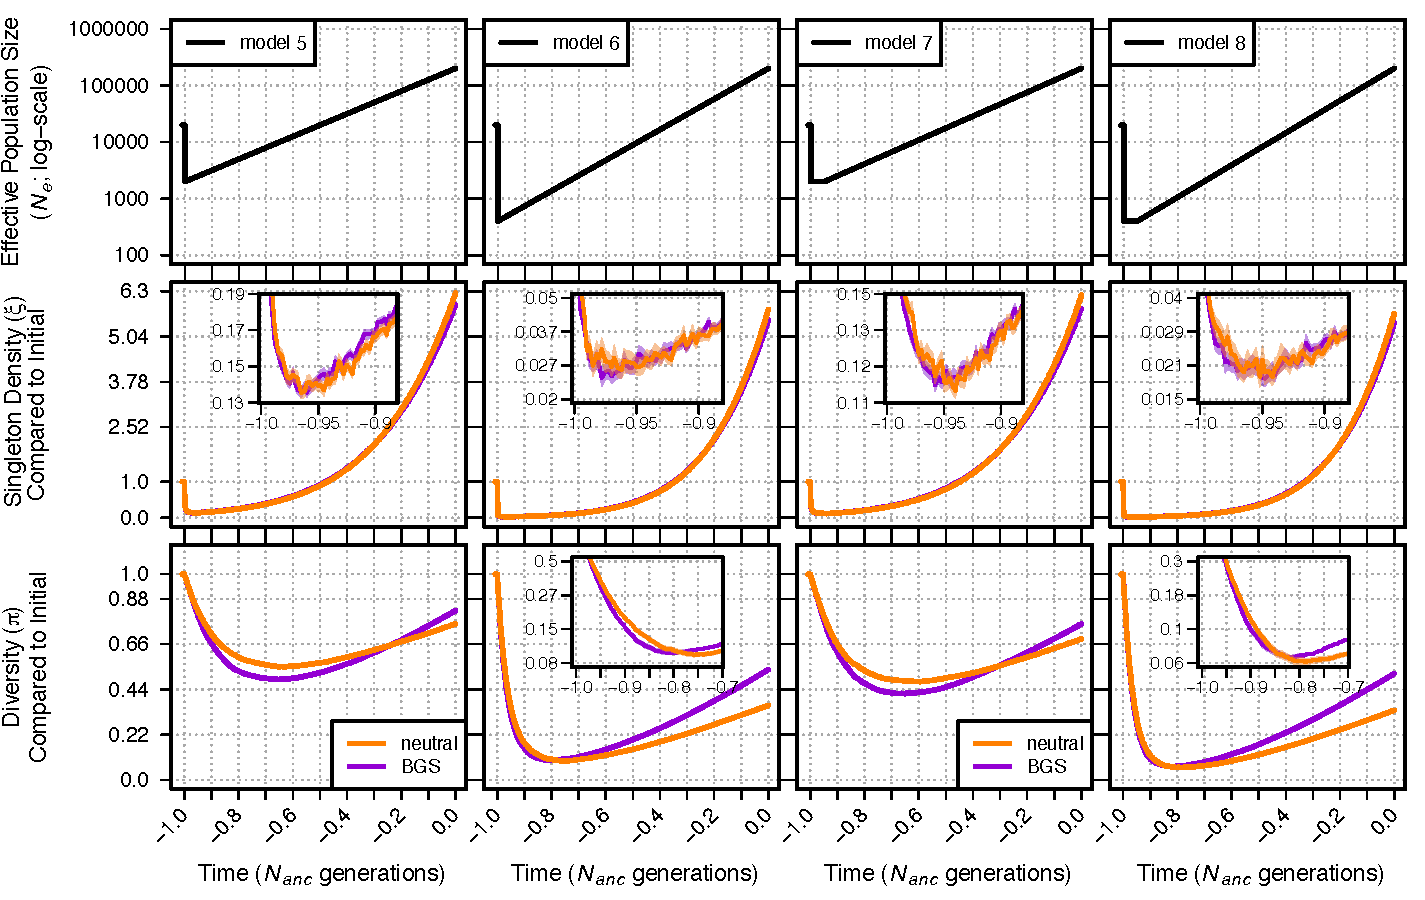
\includegraphics[width=0.8\linewidth]{figures/FigS7.pdf}
\caption{Singleton density ($\xi$ per site) and diversity ($\pi$ per site) relative to the initial generation for neutral (orange) and BGS (violet) simulations of demographic models 5-8.
The top panel shows each demographic model as in Supplemental Figure \ref{fig:S4}.
Insets show diversity over a shorter timescale and use a log scale for diversity for improved detail.
Envelopes are 95\% CIs calculated from 10,000 bootstraps of the original simulation data.
The data used for this figure is identical to that of Supplemental Figure \ref{fig:S4}.}
\label{fig:S7}
\end{figure*}
\pagebreak

\begin{figure*}[h!]
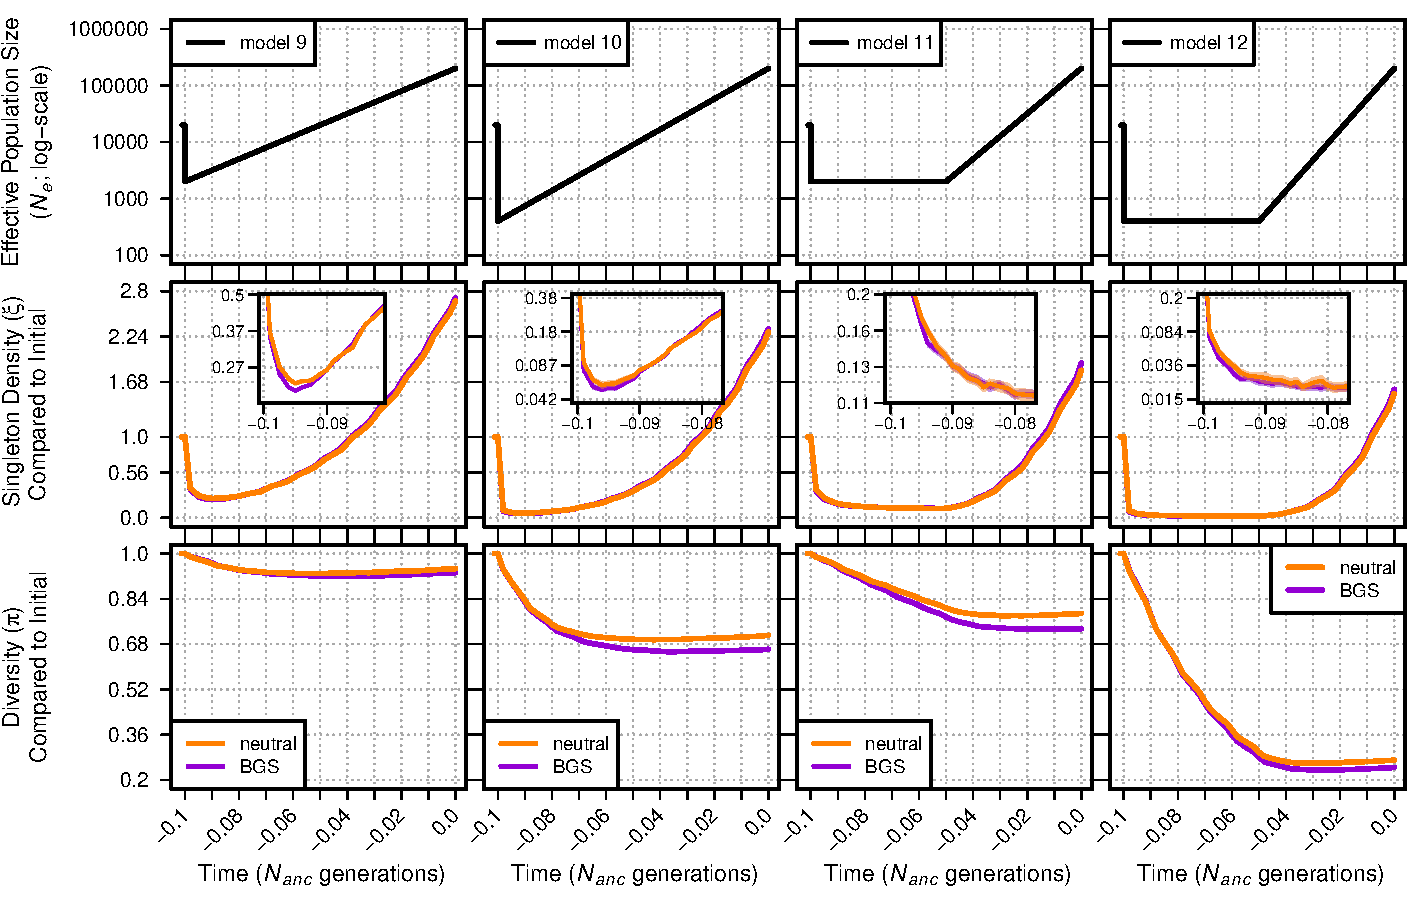
\includegraphics[width=0.8\linewidth]{figures/FigS8.pdf}
\caption{Singleton density ($\xi$ per site) and diversity ($\pi$ per site) relative to the initial generation for neutral (orange) and BGS (violet) simulations of demographic models 9-12.
The top panel shows each demographic model as in Supplemental Figure \ref{fig:S5}.
Insets show diversity over a shorter timescale and use a log scale for diversity for improved detail.
Envelopes are 95\% CIs calculated from 10,000 bootstraps of the original simulation data.
The data used for this figure is identical to that of Supplemental Figure \ref{fig:S5}.}
\label{fig:S8}
\end{figure*}
\pagebreak

\begin{figure}[]
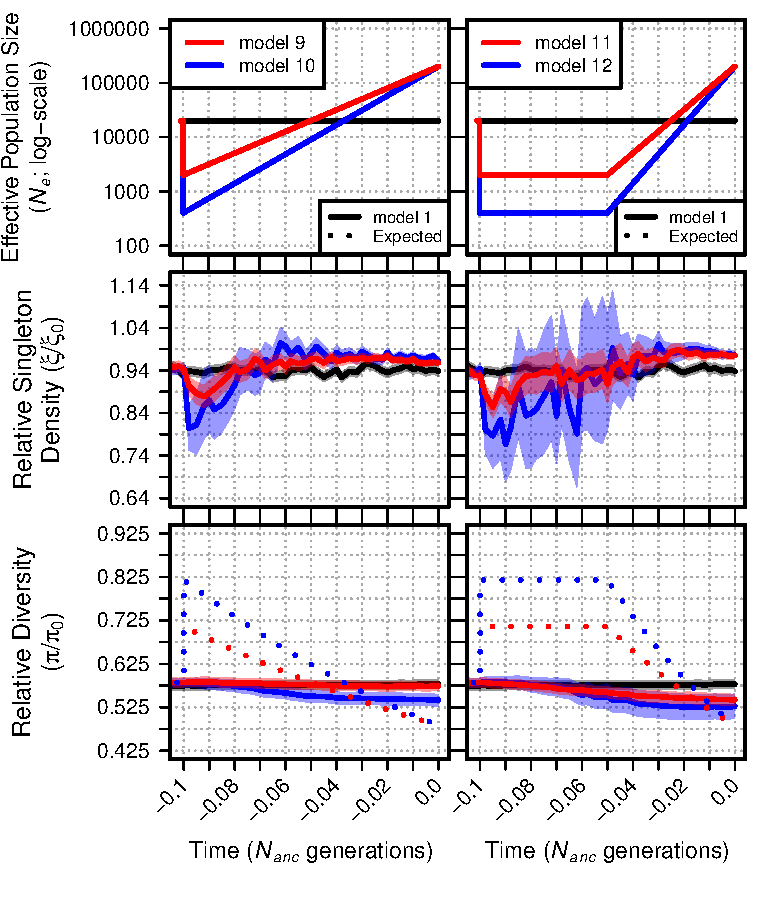
\includegraphics[width=0.5\linewidth]{figures/figsup912_newclean.pdf}
\caption{Relative singleton density ($\xi/\xi_0$) and relative diversity ($\pi/\pi_0$) across time for demographic models 1 and 9-12. The top panel shows each demographic model; time proceeds forward from left to right and is scaled by the $N_e$ of the population at the initial generation ($N_{anc}$; 20,000 individuals). Black lines show $\xi/\xi_0$ and $\pi/\pi_0$ from simulations of a constant sized population (model 1). Dotted lines in the bottom panel show the equilibrium expectation of $\pi/\pi_0$ from  \citet{nordborg1996effect} given the specific selection parameters and the instantaneous $N_e$ at each time point. Envelopes are 95\% CIs calculated from 10,000 bootstraps of the original simulation data.}
\label{fig:S912}
\end{figure}
\pagebreak

\begin{figure}[htb]
    \centering
    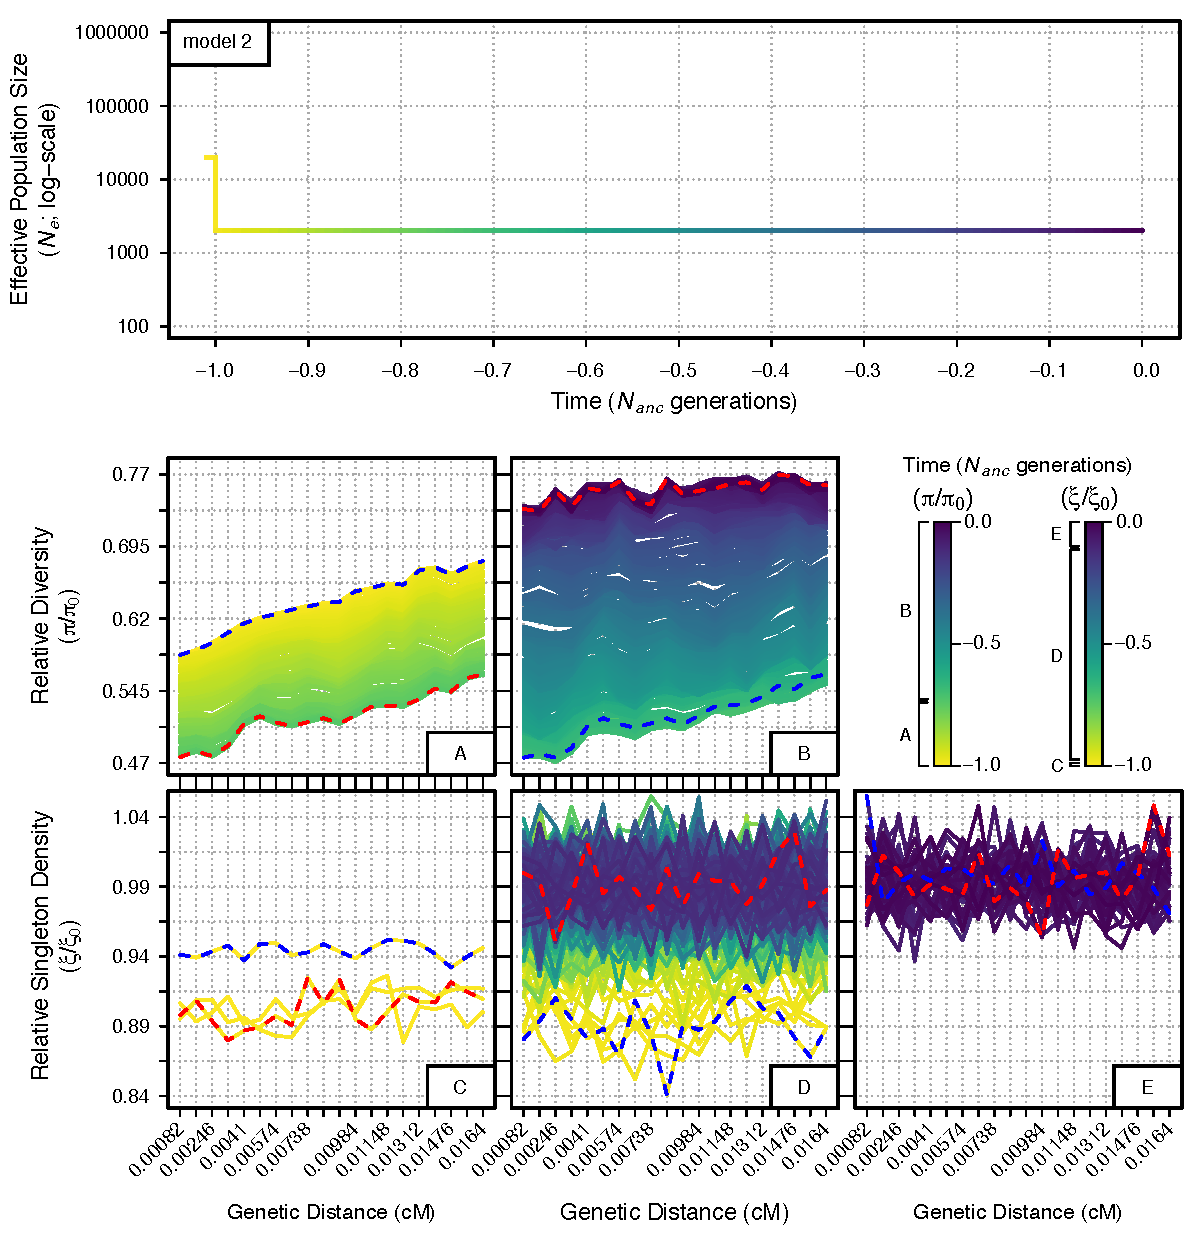
\includegraphics[width=\linewidth]{figures/FigS10.pdf}
\end{figure}
\begin{figure}[htb]\ContinuedFloat
    \centering
    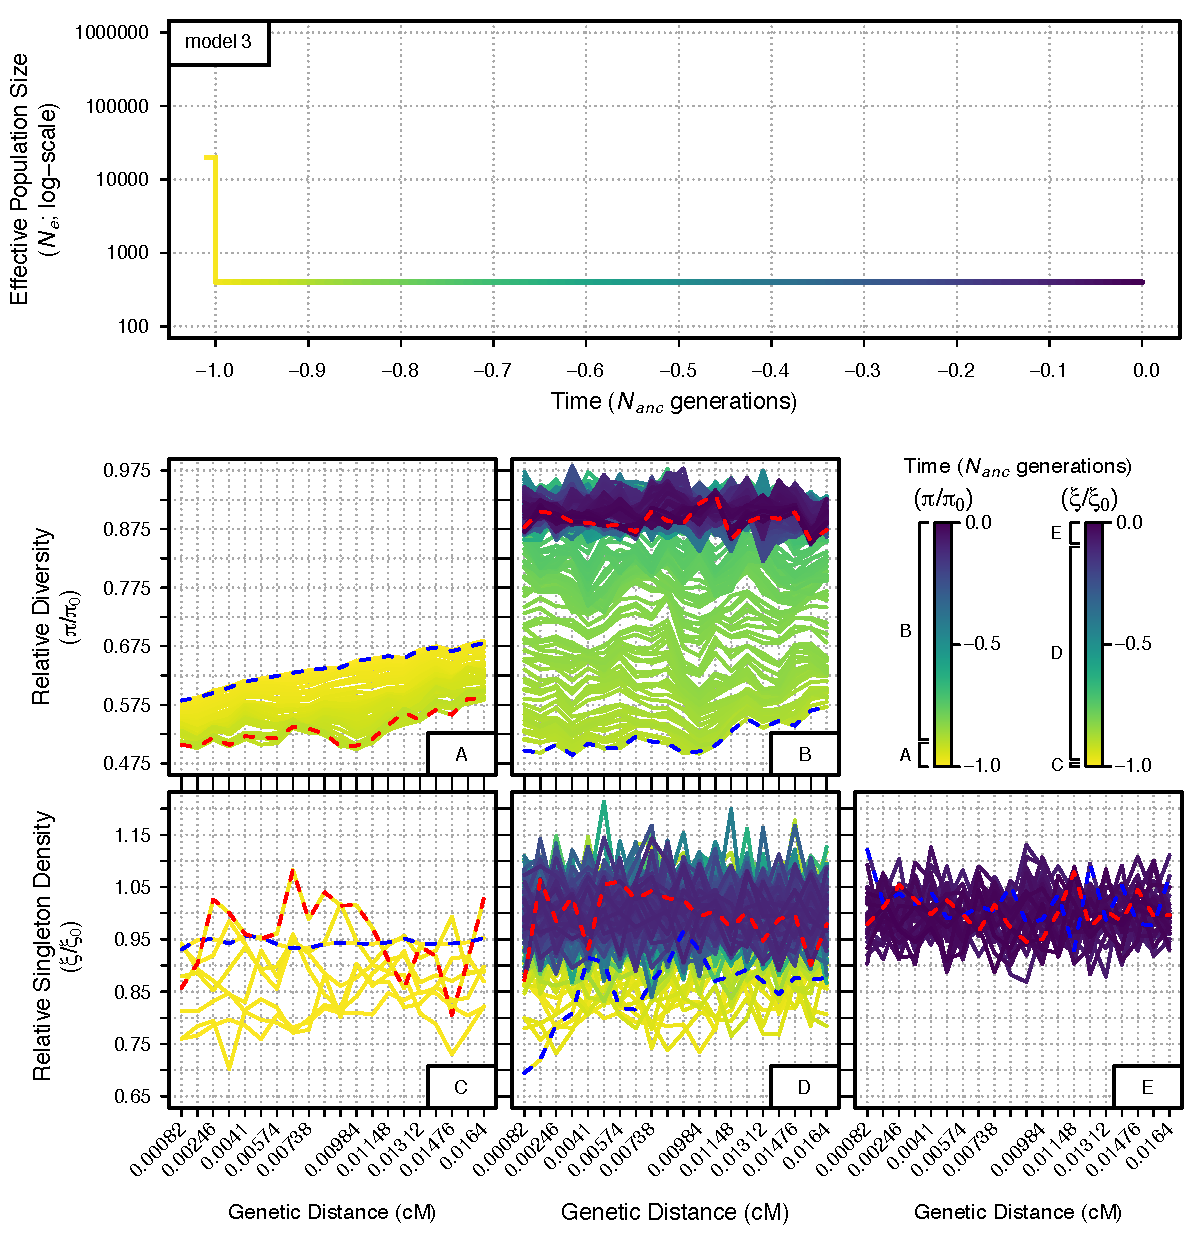
\includegraphics[width=\linewidth]{figures/FigS11.pdf}
\end{figure}
\begin{figure}[htb]\ContinuedFloat
    \centering
    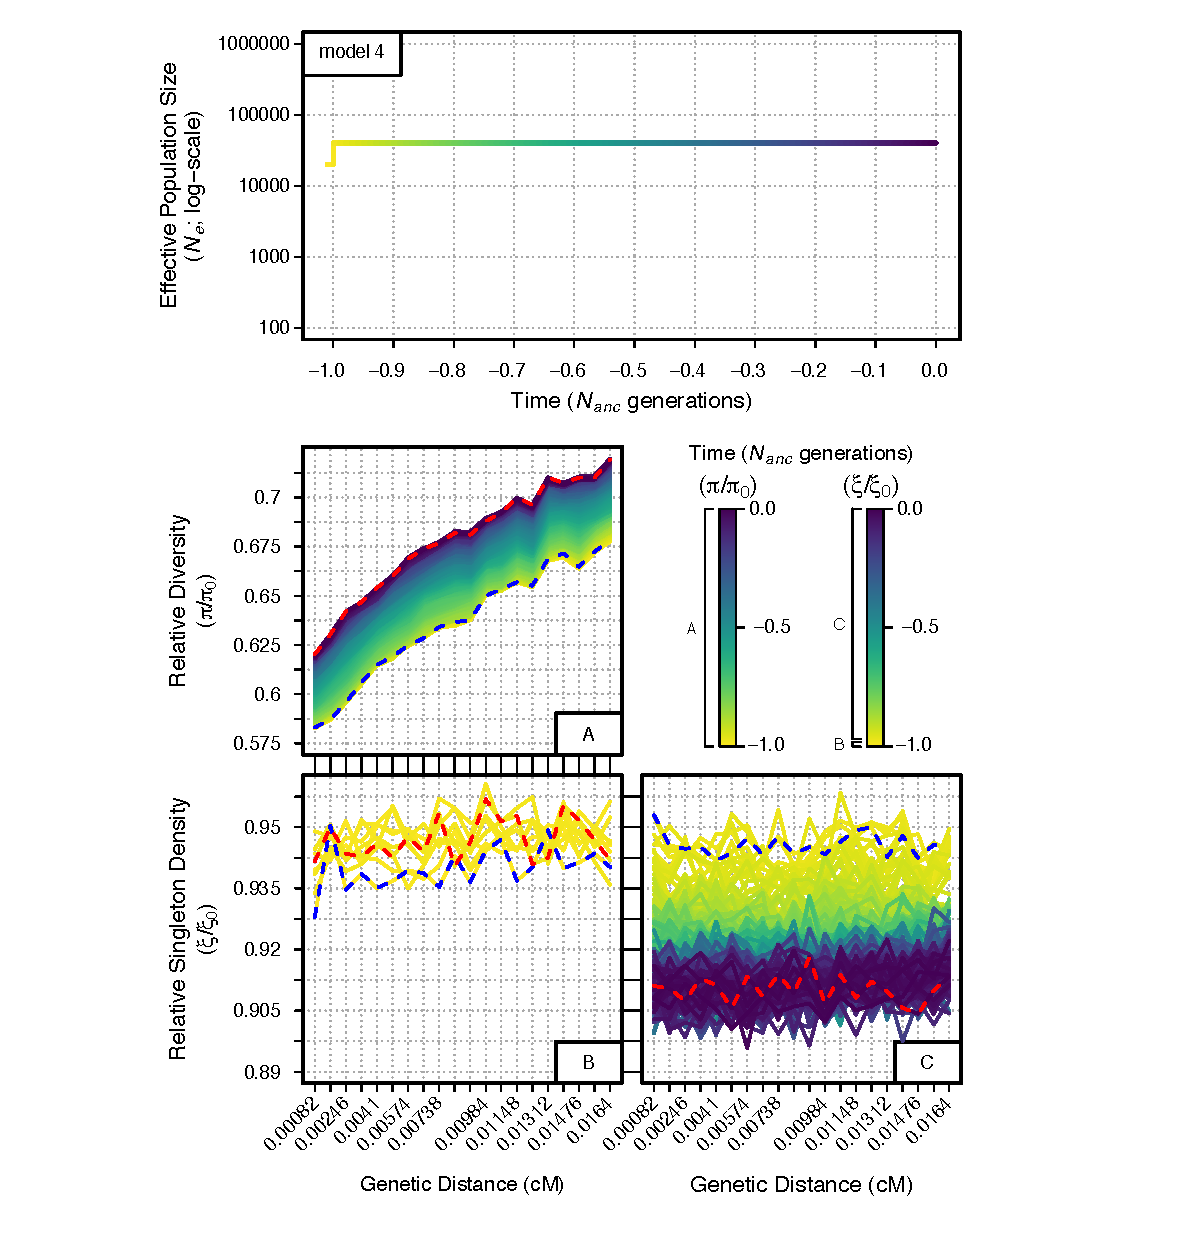
\includegraphics[width=\linewidth]{figures/FigS12.pdf}
\end{figure}
\begin{figure}[htb]\ContinuedFloat
    \centering
    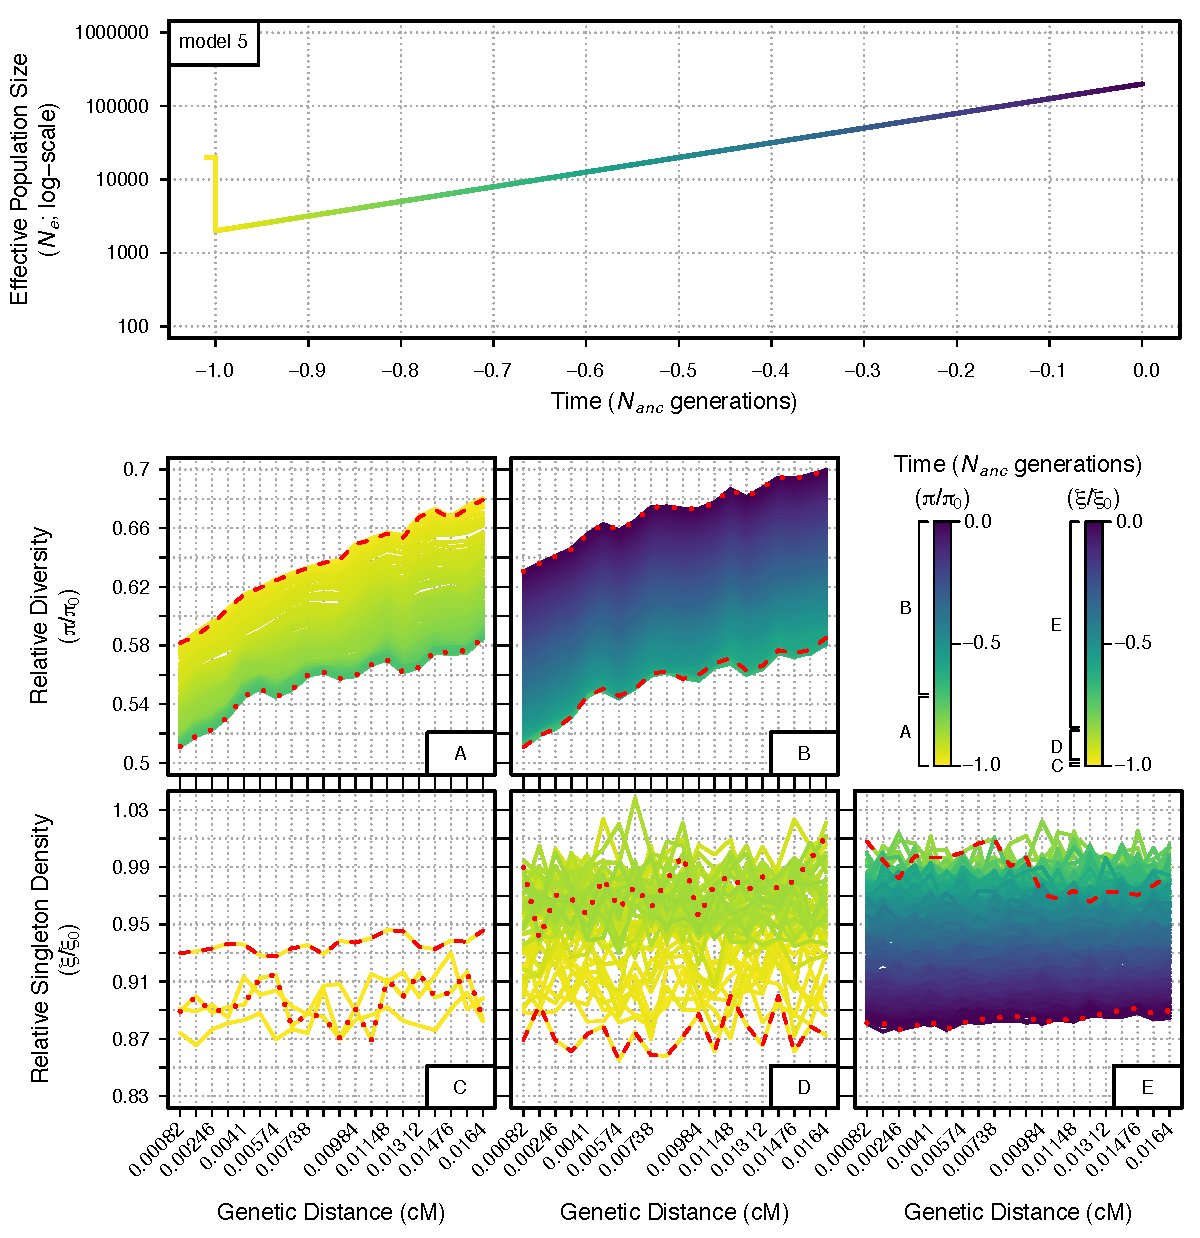
\includegraphics[width=\linewidth]{figures/FigS13.pdf}
\end{figure}
\begin{figure}[htb]\ContinuedFloat
    \centering
    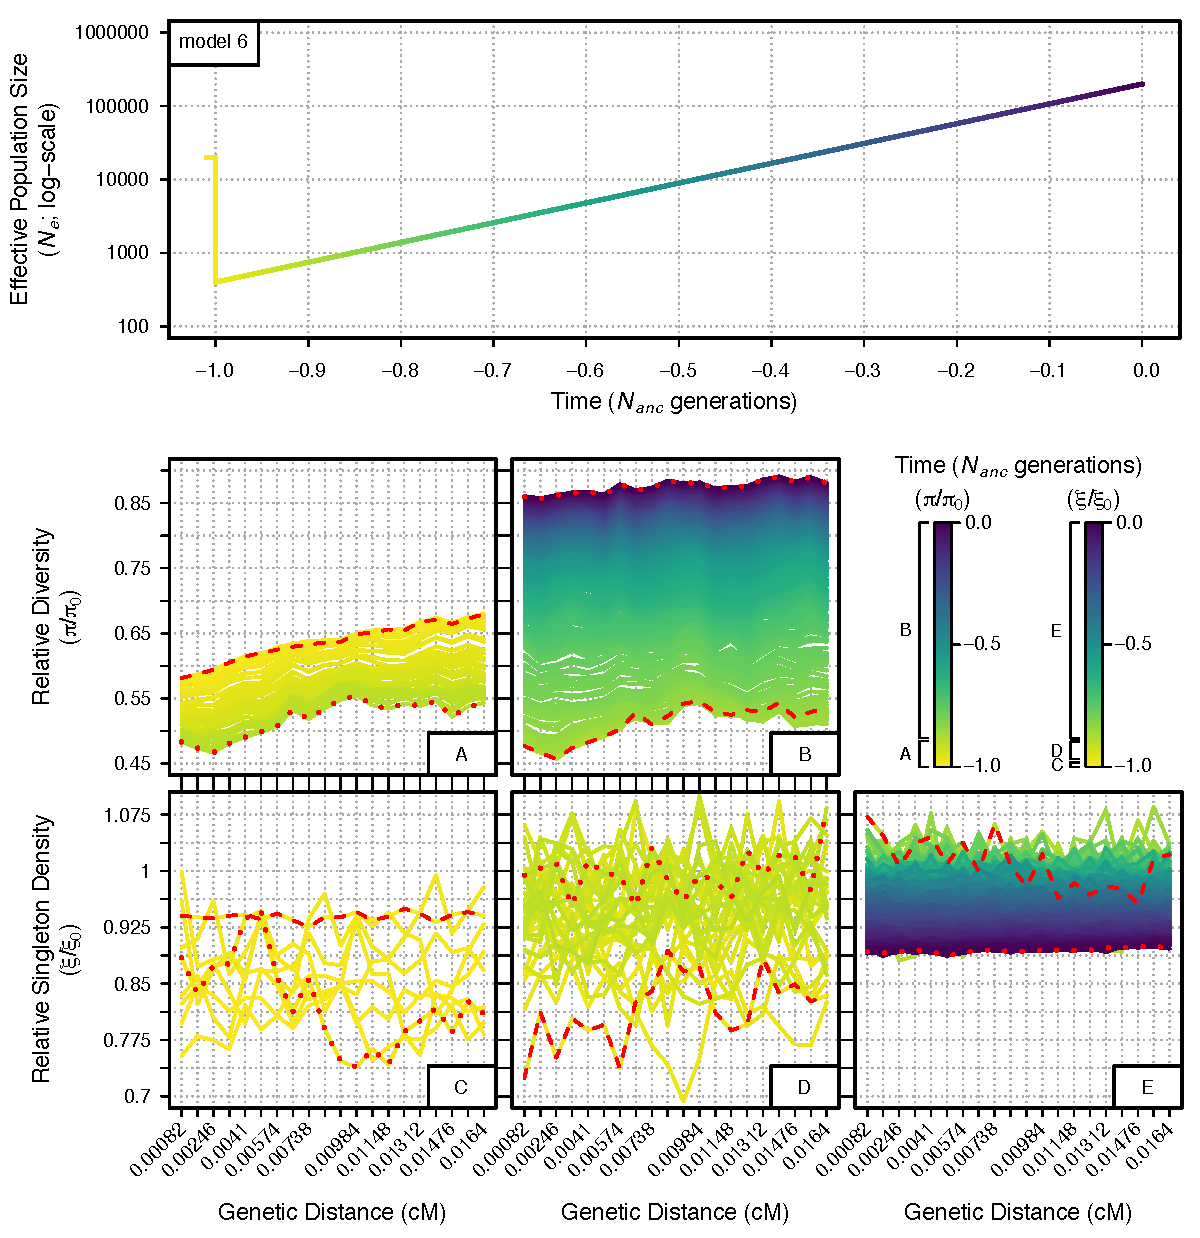
\includegraphics[width=\linewidth]{figures/FigS14.pdf}
\end{figure}
\begin{figure}[htb]\ContinuedFloat
    \centering
    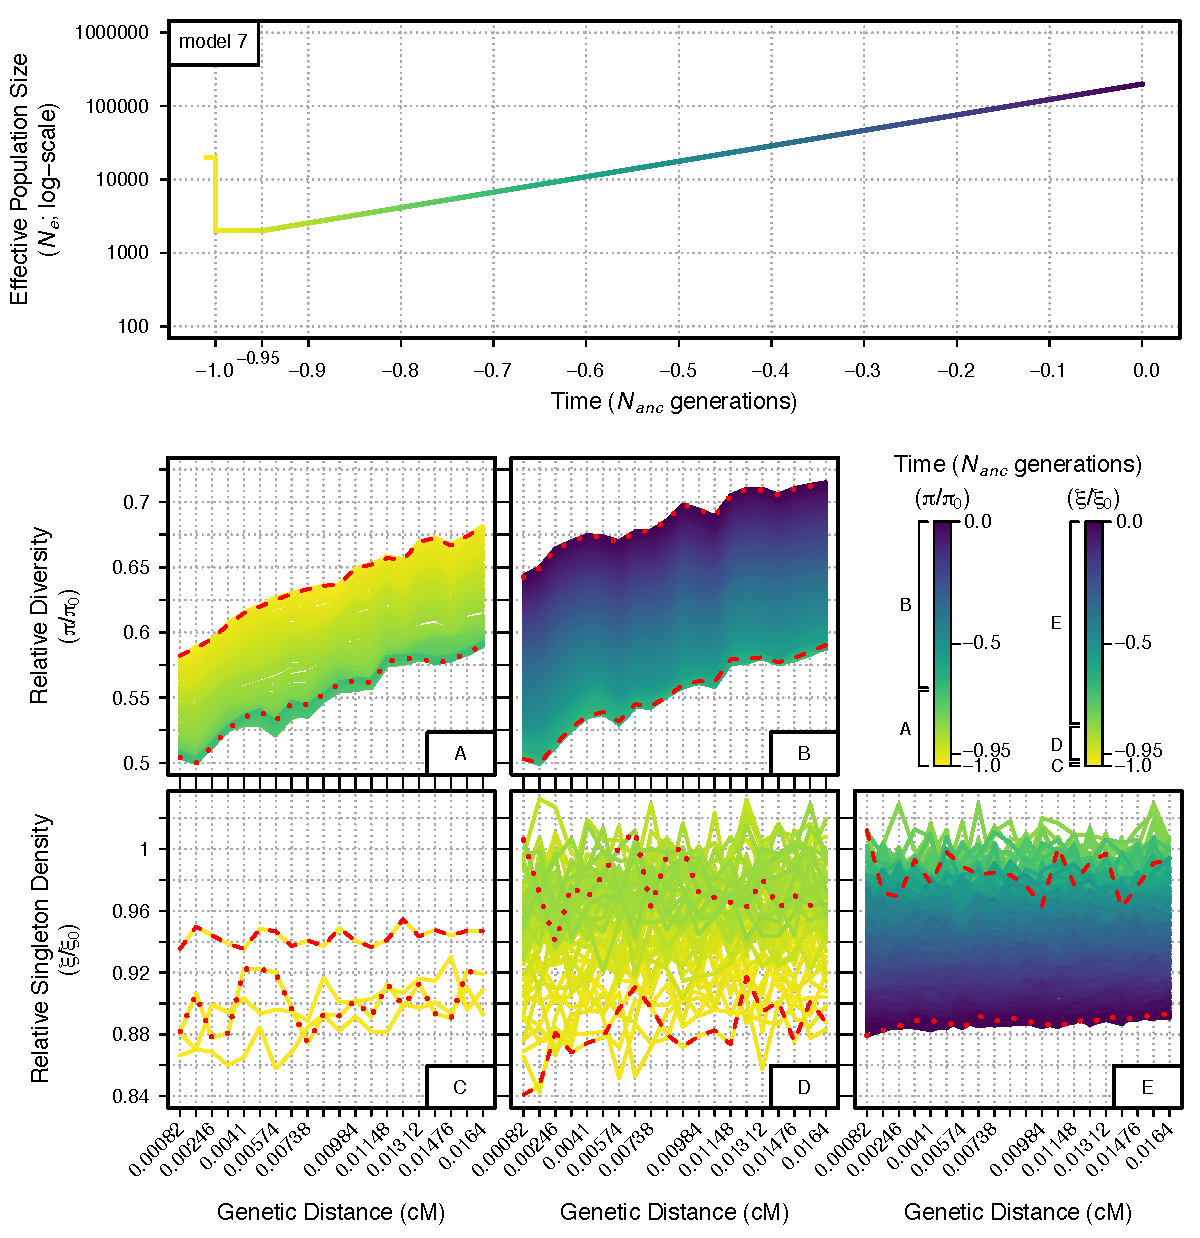
\includegraphics[width=\linewidth]{figures/FigS15.pdf}
\end{figure}
\begin{figure}[htb]\ContinuedFloat
    \centering
    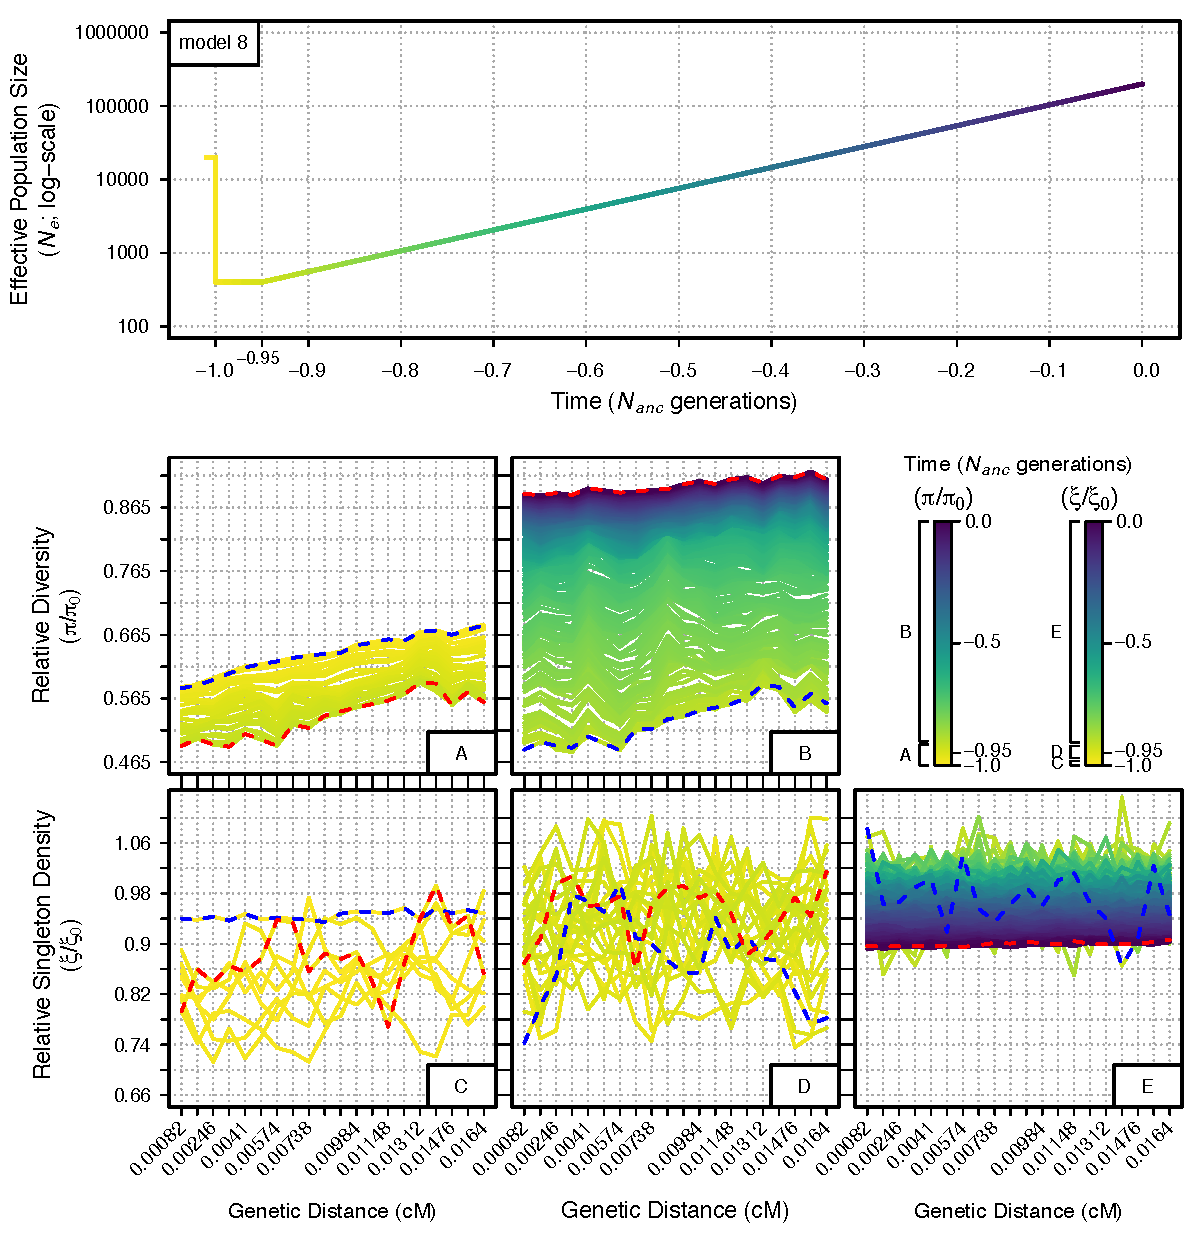
\includegraphics[width=\linewidth]{figures/FigS16.pdf}
\end{figure}
\begin{figure}[htb]\ContinuedFloat
    \centering                   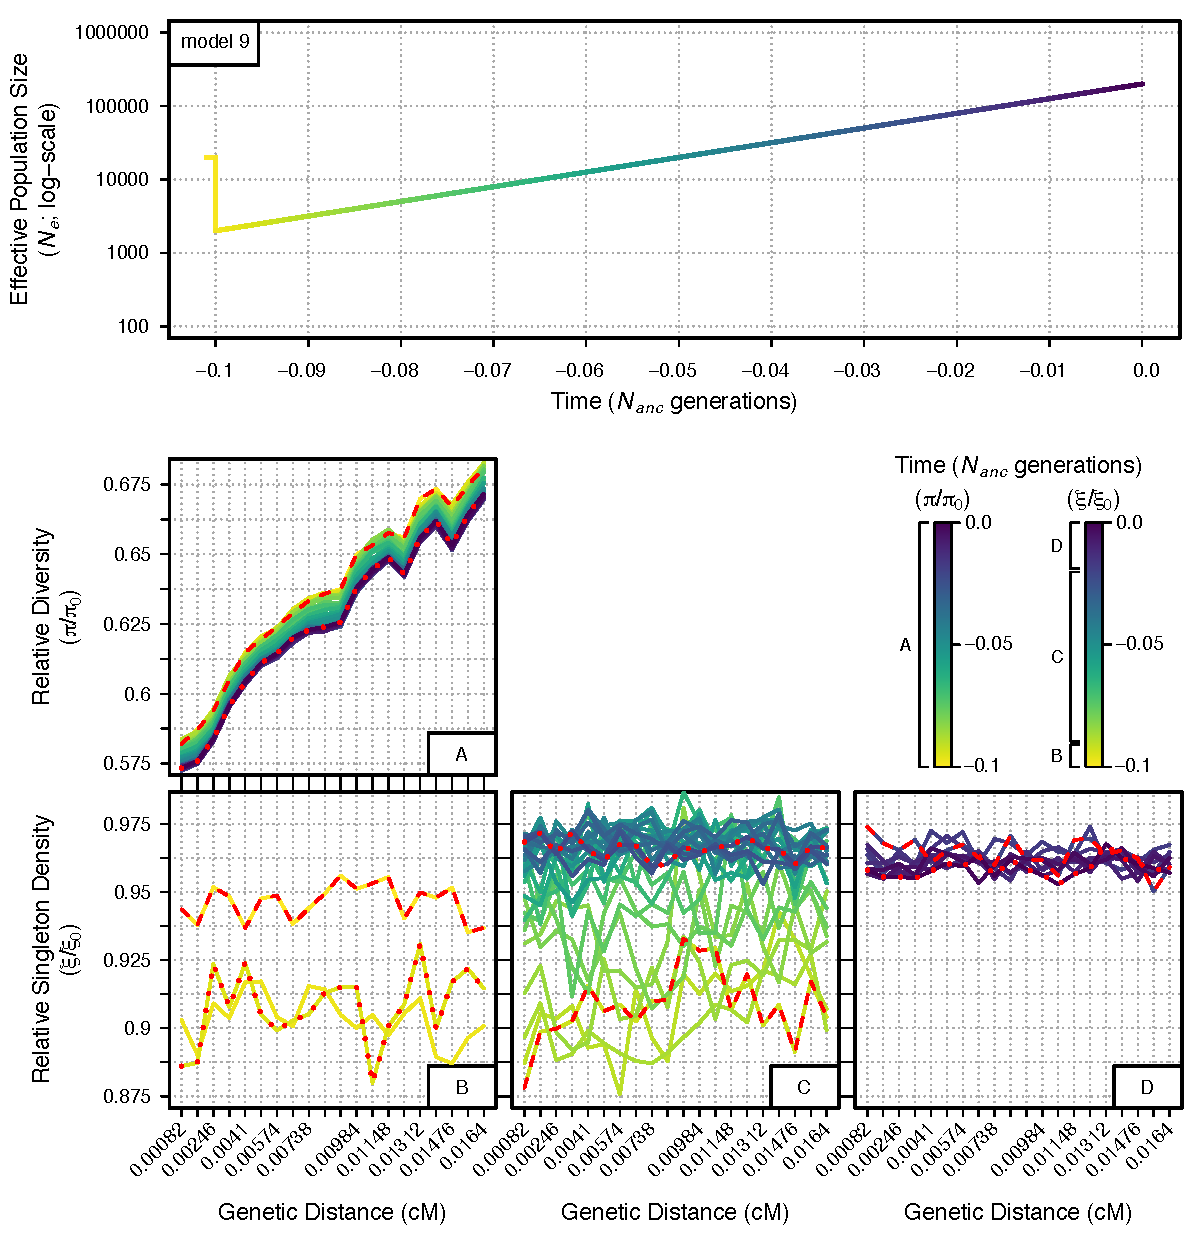
\includegraphics[width=\linewidth]{figures/FigS17.pdf}
\end{figure}
\begin{figure}[htb]\ContinuedFloat
      \centering
      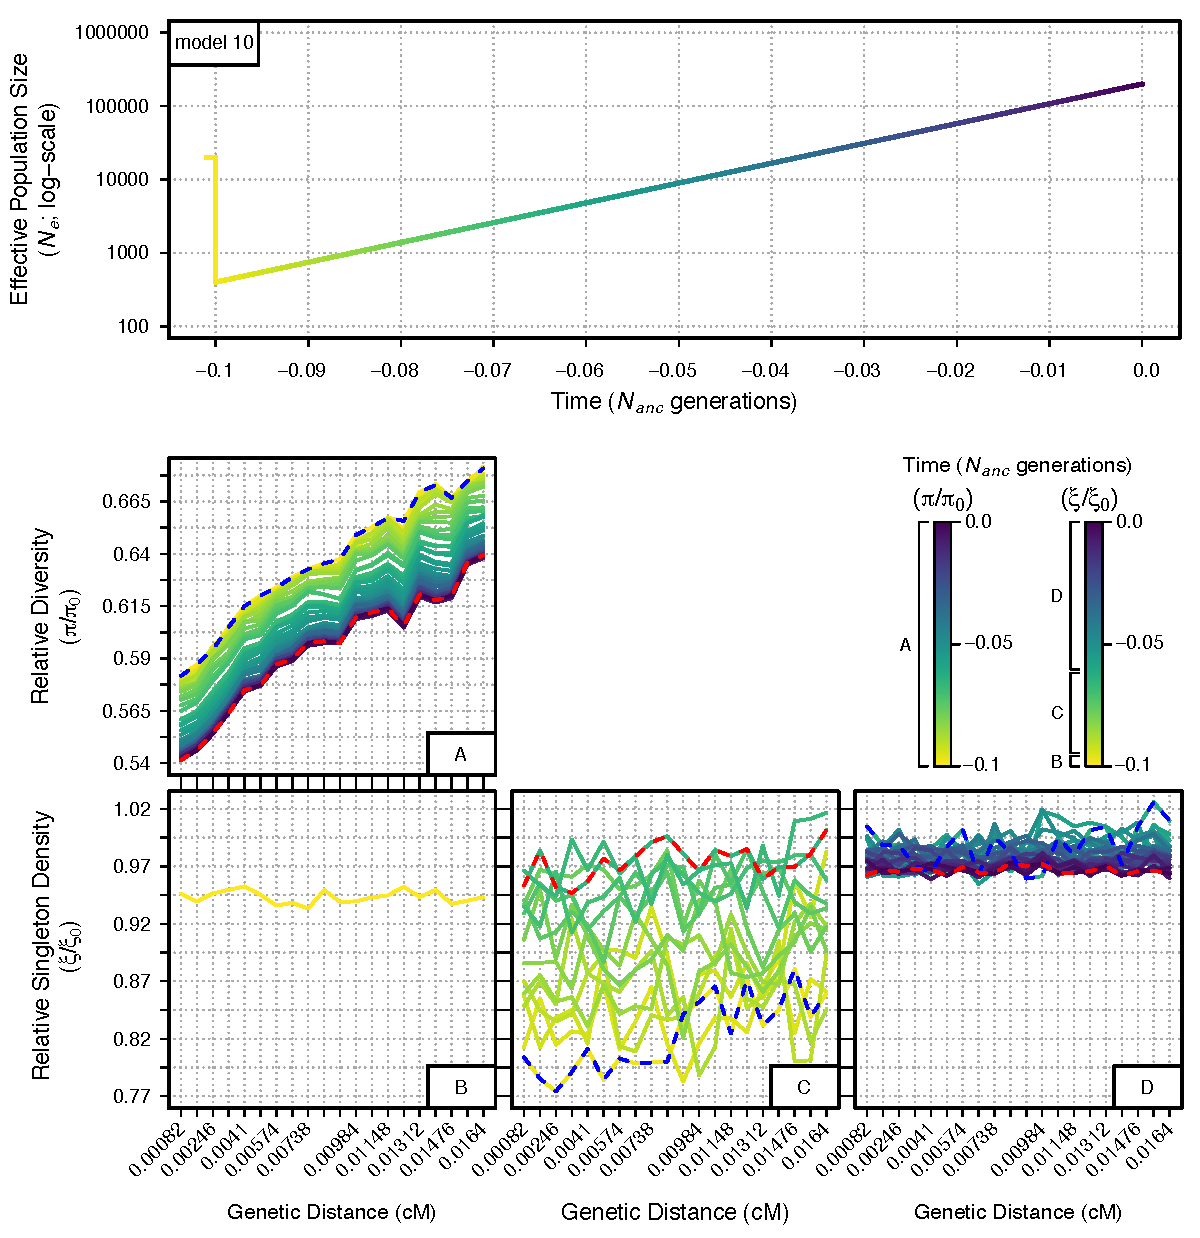
\includegraphics[width=\linewidth]{figures/FigS18.pdf}
\end{figure}
\begin{figure}[htb]\ContinuedFloat
      \centering
      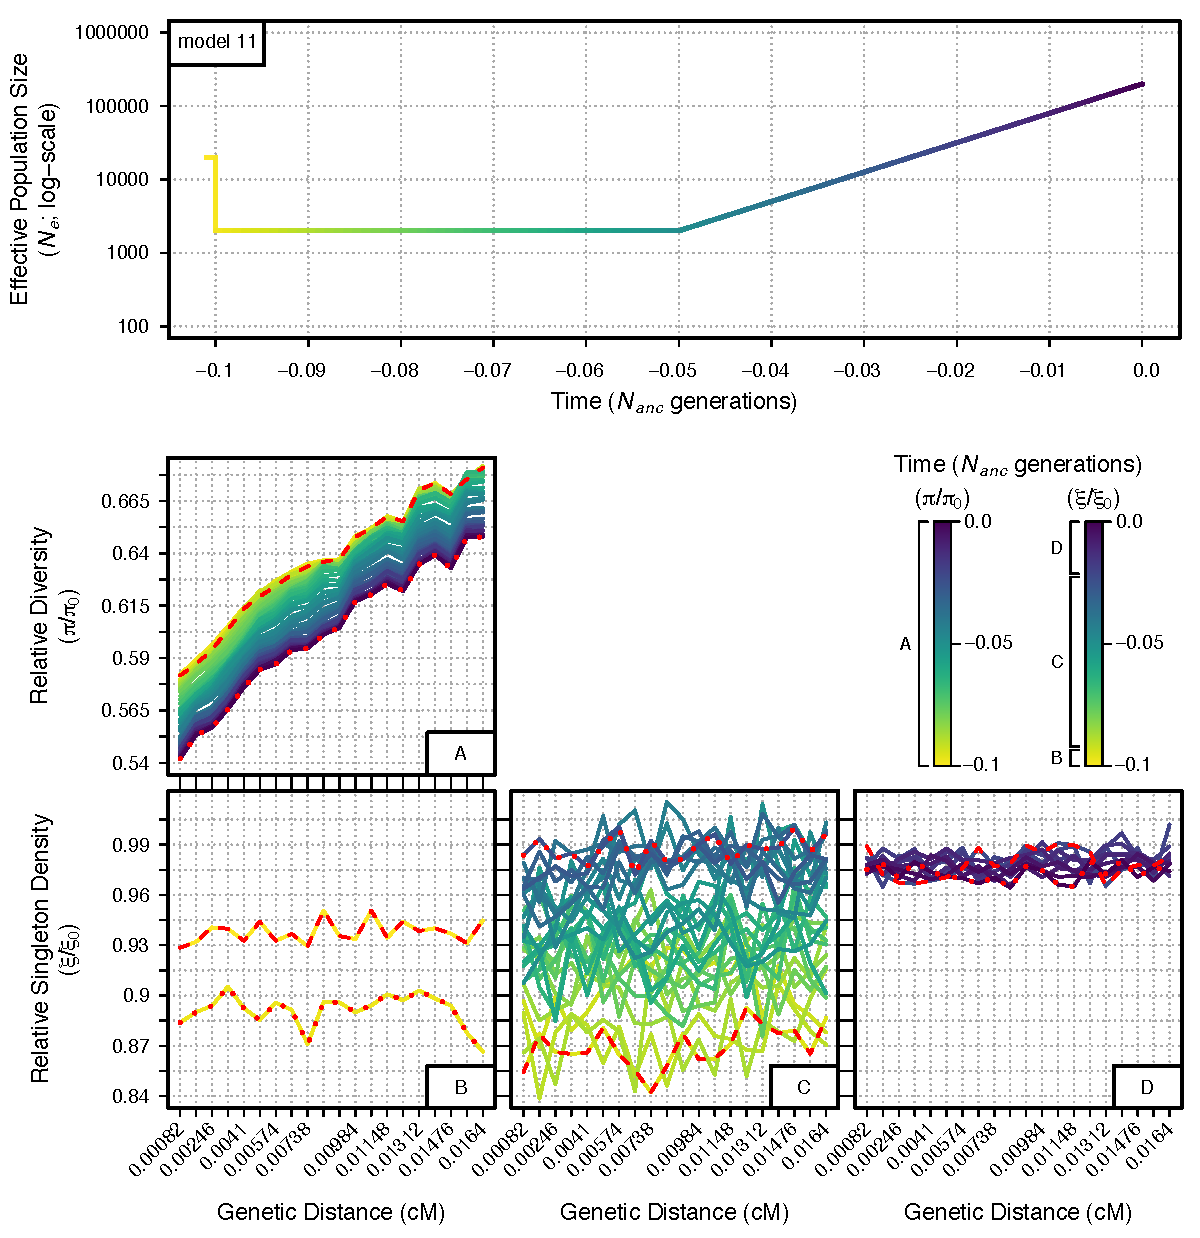
\includegraphics[width=\linewidth]{figures/FigS19.pdf}
\end{figure}
\begin{figure}[htb]
      \centering
      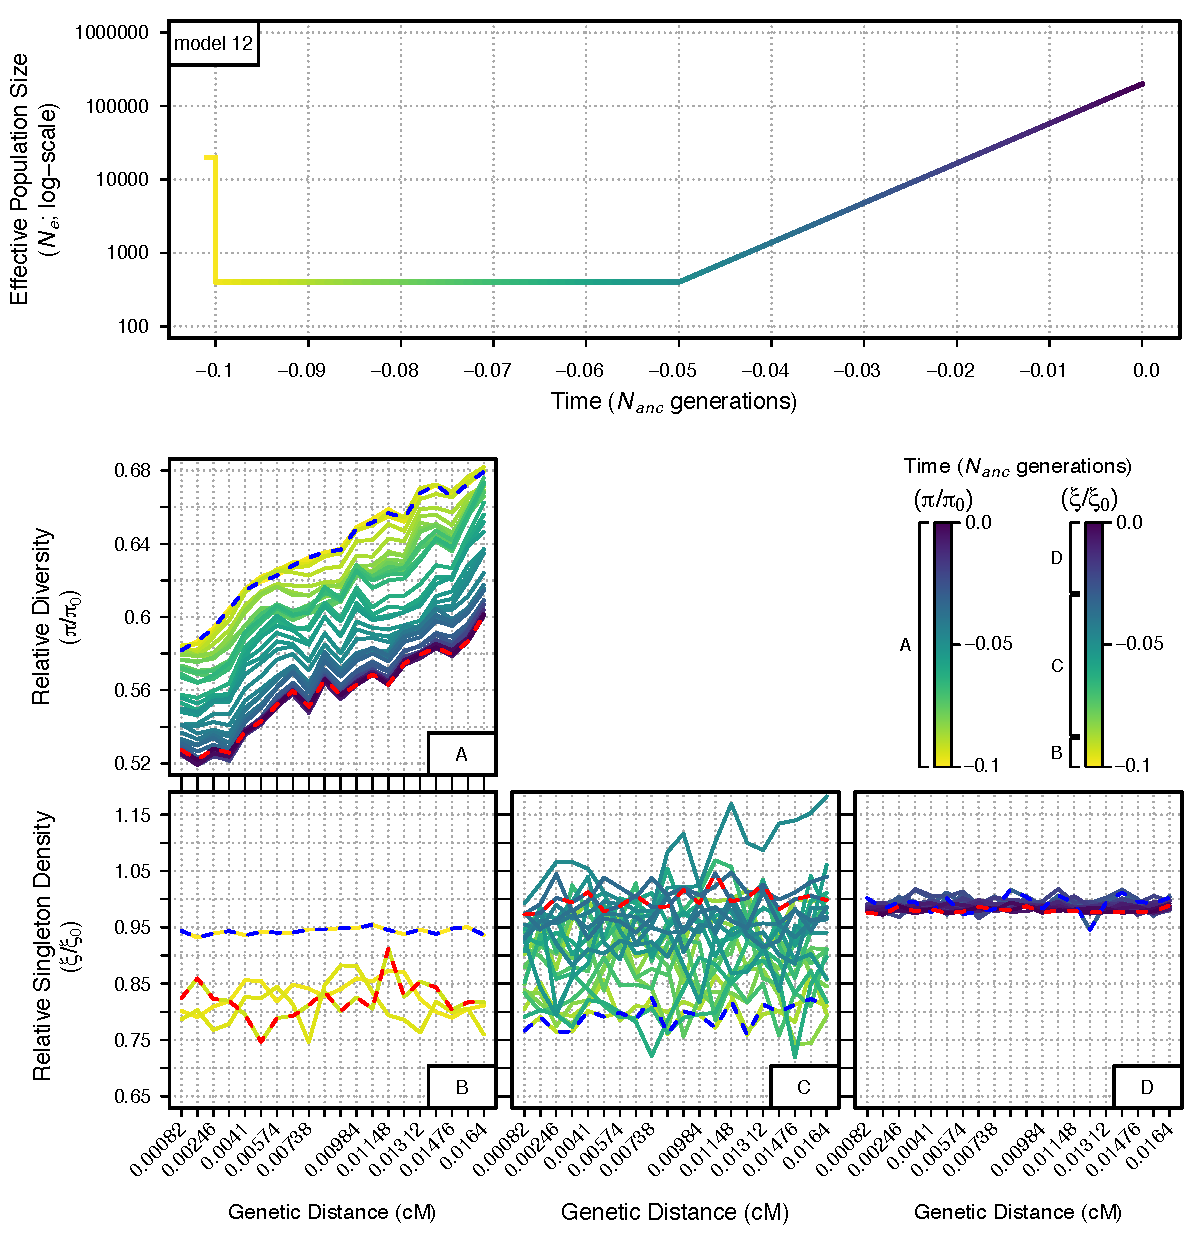
\includegraphics[width=\linewidth]{figures/FigS20.pdf}
      \caption{Relative diversity ($\pi/\pi_0$) and singleton density ($\xi/\xi_0$) through time for demographic models 2-12 measured across a neutral 200 kb region under the effects of BGS.
The genetic distance of each 10 kb bin from the selected locus is indicated on the x-axes of the bottom two panels, with genetic distance increasing from left to right.
Each line measuring $\pi/\pi_0$ and $\xi/\xi_0$ across the 200 kb neutral region represents a specific generation of the demographic model (401 discrete generations for demographic models 2-8, 41 discrete generations for demographic models 9-12).
Specific generations are indicated by the color of the demographic model at the top of each figure (time is scaled in units of $N_{anc}$ generations [20,000 individuals]) and in the figure legend.
When necessary, multiple plots are given for $\pi/\pi_0$ and $\xi/\xi_0$ in order to prevent overlap of the measurements between generations (see legend for specific generations covered in each plot).
Red dashed lines and red dotted lines indicate the first generation and last generation measured, respectively, for each specific plot.}
\label{fig:all200}
\end{figure}
\pagebreak

% \begin{table*}[htbp]
% \centering

% \caption{\bf Shrink a large table to fit the page}
% %\begin{adjustbox}{totalheight=\textheight-2\baselineskip}
% \begin{tableminipage}{\textwidth}
% \begin{small}
% \begin{tabularx}{\textwidth}{sb}
% \hline
% Parameter & Description \\
% \hline
% \textbf{Adaptation} & \textbf{Trait related parameters} \\
% \hline
% Time to optimum & Generations until new optimum is reached \\
% Adaptation rate (haldane) & Adaptation rate until new optimum is reached. Calculated as $rate(h) = \frac{\frac{ln(x_2)}{sd_{x_{12}}}-\frac{ln(x_1)}{sd_{x_{12}}}}{t_2-t_1}$ \\
% Final genetic variance & Genetic variance in the final generation \\
% \textbf{Fixations} & \textbf{Mutations that fix after the optimum shift} \\
% \hline
% From new mutations (\#) & Sum of fixed mutations in the final population that were already segregating before  the optimum shift \\
% From standing variation (\#) & Sum of fixed mutations in the final population that arose after the optimum shift \\
% Max. effect size & Maximal effect size of all fixations \\
% Mean effect size & Mean effect size of all fixations \\
% Mean effect size of negative fixations & Mean effect size of negative mutations \\
% Mean effect size of positive fixations & Mean effect size of positive mutations \\
% Mean emergence time & Mean generation when a mutation arose that fixed in the last 0.1 N generations \\
% Mean fixation time & Mean generation in which a mutation fixed \\
% Min. effect size & Minimal effect size of all fixations \\
% Negative (\#) & Sum of fixed mutations with negative effects in the final population \\
% New/standing fixations & Ratio of mutations from new mutations vs. standing mutations  \\
% Proportion negative & Proportion of negative fixations from all mutations \\
% Positive (\#) & Sum of fixed mutations with positive effects in the final population \\
% SD of effect sizes & Standard deviation of effect sizes of all fixations \\
% SD of negative effect sizes & Standard deviation of effect sizes of negative fixations \\
% SD of positive effect sizes & Standard deviation of effect sizes of positive fixations \\
% Total (\#) & Sum of fixed mutations in the final population \\
% \textbf{Sweeps} & \textbf{Mutations that fix faster than 99\% of neutral fixations} \\
% \hline
% Hard sweeps (\#) & Sum of selective sweeps from new mutations \\
% Proportion of hard sweeps & Porportion of hard selective sweeps of all selective sweeps \\
% Proportion of sweeps from standing & Proportion of selective sweeps from stainding variation of all selection sweeps \\
% Sweeps (\#) & Sum of selective sweeps \\
% Sweeps from standing variation (\#) & Sum of selective sweeps from mutations that were already segregating before  the optimum shift \\
% Sweeps/fixations & Ratio of sweeps vs. fixations \\
% \textbf{Segregating sites} & \textbf{Mutations that segregate in the final generation} \\
% \hline
% Max. effect size & Maximal effect size of segregating sites \\
% Mean effect size & Mean effect size of segregating sites \\
% Mean effect size of negative sites & Mean effect size of segregating sites with negative effects \\
% Mean effect size of positive sites & Mean effect size of segregating sites with positive effects \\
% Mean frequency of all sites & Mean allele frequency of segregating sites \\
% Mean frequency of negative sites & Mean allele frequency of segregating sites with negative effects \\
% Mean frequency of positive sites & Mean allele frequency of segregating sites with positive effects \\
% Min. effect size & Minimal effect size of segregating sites \\
% Negative (\#) & Sum of segregating sites with negative effect \\
% Positive (\#) & Sum of segregating sites with positive effect \\
% Proportion of negative sites & Proportion of segregating sites with negative effect of all segregating sites \\
% Standard deviation of effect sizes & Standard deviation of effect sizes of all segregating sites \\
% Total (\#) & Sum segregating sites in the final generation \\
% \hline

% \end{tabularx}
%   \label{tab:parameter_list}
%   \end{small}
% \end{tableminipage}

% %\end{adjustbox}
% \end{table*}


\end{document}
